\documentclass[twoside,11pt]{article}

% +
%  Name:
%     sc16.tex

%  Purpose:
%     Starlink Cookbook dealing with IFU data product analysis (SC/16)

%  Authors:
%     AALLAN: Alasdair Allan (Starlink, University of Exeter)

%  Copyright:
%     Copyright (C) 1997-2001 Particle Physics and Astronomy
%     Research Council. All Rights Reserved.
%
%  History:
%     01-SEP-2000 (AALLAN) 
%        Original version.
%     24-NOV_2000 (AALLAN)
%        Added VIMOS information
%     30-DEC-2000 (AALLAN)
%        Cleanup for release
%     02-JAN-2001 (AALLAN)
%        Release version

%-

% ? Specify used packages
\usepackage{graphicx}        %  Use this one for final production.
% \usepackage[draft]{graphicx} %  Use this one for drafting.
% ? End of specify used packages

\pagestyle{myheadings}

% -----------------------------------------------------------------------------
% ? Document identification
% Fixed part
\newcommand{\stardoccategory}  {STARLINK Cookbook}
\newcommand{\stardocinitials}  {SC}
\newcommand{\stardocsource}    {sc\stardocnumber}

% Variable part - replace [xxx] as appropriate.
\newcommand{\stardocnumber}    {16.1-1}
\newcommand{\stardocauthors}   {A.~Allan}
\newcommand{\stardocdate}      {30th September 2002}
\newcommand{\stardoctitle}     {The IFU Data Product Cookbook}
\newcommand{\stardocabstract}
{This cookbook is a collection of material covering IFU data reduction and analysis. Along with this material are pointers to more advanced documents dealing with the various packages, and hints and tips about how to deal with commonly occurring problems.}

% ? End of document identification
% -----------------------------------------------------------------------------

% +
%  Name:
%     sc.tex
%
%  Purpose:
%     Template for Starlink Cookbook (SC) documents.
%     Refer to SUN/199
%
%  Authors:
%     AJC: A.J.Chipperfield (Starlink, RAL)
%     BLY: M.J.Bly (Starlink, RAL)
%
%  History:
%     16-JUN-1997 (BLY):
%        Original, based on SUN/SG templates.
%     {Add further history here}
%
% -

\newcommand{\stardocname}{\stardocinitials /\stardocnumber}
\markboth{\stardocname}{\stardocname}
\setlength{\textwidth}{160mm}
\setlength{\textheight}{230mm}
\setlength{\topmargin}{-2mm}
\setlength{\oddsidemargin}{0mm}
\setlength{\evensidemargin}{0mm}
\setlength{\parindent}{0mm}
\setlength{\parskip}{\medskipamount}
\setlength{\unitlength}{1mm}

% -----------------------------------------------------------------------------
%  Hypertext definitions.
%  ======================
%  These are used by the LaTeX2HTML translator in conjunction with star2html.

%  Comment.sty: version 2.0, 19 June 1992
%  Selectively in/exclude pieces of text.
%
%  Author
%    Victor Eijkhout                                      <eijkhout@cs.utk.edu>
%    Department of Computer Science
%    University Tennessee at Knoxville
%    104 Ayres Hall
%    Knoxville, TN 37996
%    USA

%  Do not remove the %\begin{rawtex} and %\end{rawtex} lines (used by 
%  star2html to signify raw TeX that latex2html cannot process).
%\begin{rawtex}
\makeatletter
\def\makeinnocent#1{\catcode`#1=12 }
\def\csarg#1#2{\expandafter#1\csname#2\endcsname}

\def\ThrowAwayComment#1{\begingroup
    \def\CurrentComment{#1}%
    \let\do\makeinnocent \dospecials
    \makeinnocent\^^L% and whatever other special cases
    \endlinechar`\^^M \catcode`\^^M=12 \xComment}
{\catcode`\^^M=12 \endlinechar=-1 %
 \gdef\xComment#1^^M{\def\test{#1}
      \csarg\ifx{PlainEnd\CurrentComment Test}\test
          \let\html@next\endgroup
      \else \csarg\ifx{LaLaEnd\CurrentComment Test}\test
            \edef\html@next{\endgroup\noexpand\end{\CurrentComment}}
      \else \let\html@next\xComment
      \fi \fi \html@next}
}
\makeatother

\def\includecomment
 #1{\expandafter\def\csname#1\endcsname{}%
    \expandafter\def\csname end#1\endcsname{}}
\def\excludecomment
 #1{\expandafter\def\csname#1\endcsname{\ThrowAwayComment{#1}}%
    {\escapechar=-1\relax
     \csarg\xdef{PlainEnd#1Test}{\string\\end#1}%
     \csarg\xdef{LaLaEnd#1Test}{\string\\end\string\{#1\string\}}%
    }}

%  Define environments that ignore their contents.
\excludecomment{comment}
\excludecomment{rawhtml}
\excludecomment{htmlonly}
%\end{rawtex}

%  Hypertext commands etc. This is a condensed version of the html.sty
%  file supplied with LaTeX2HTML by: Nikos Drakos <nikos@cbl.leeds.ac.uk> &
%  Jelle van Zeijl <jvzeijl@isou17.estec.esa.nl>. The LaTeX2HTML documentation
%  should be consulted about all commands (and the environments defined above)
%  except \xref and \xlabel which are Starlink specific.

\newcommand{\htmladdnormallinkfoot}[2]{#1\footnote{#2}}
\newcommand{\htmladdnormallink}[2]{#1}
\newcommand{\htmladdimg}[1]{}
\newenvironment{latexonly}{}{}
\newcommand{\hyperref}[4]{#2\ref{#4}#3}
\newcommand{\htmlref}[2]{#1}
\newcommand{\htmlimage}[1]{}
\newcommand{\htmladdtonavigation}[1]{}

%  Starlink cross-references and labels.
\newcommand{\xref}[3]{#1}
\newcommand{\xlabel}[1]{}

%  LaTeX2HTML symbol.
\newcommand{\latextohtml}{{\bf LaTeX}{2}{\tt{HTML}}}

%  Define command to re-centre underscore for Latex and leave as normal
%  for HTML (severe problems with \_ in tabbing environments and \_\_
%  generally otherwise).
\newcommand{\latex}[1]{#1}
\newcommand{\setunderscore}{\renewcommand{\_}{{\tt\symbol{95}}}}
\latex{\setunderscore}

%  Redefine the \tableofcontents command. This procrastination is necessary 
%  to stop the automatic creation of a second table of contents page
%  by latex2html.
\newcommand{\latexonlytoc}[0]{\tableofcontents}

% Figure environment. Defined for latex2html. #1 is postscript file
% #2 the qualifiers, #3 the gif file, #4 the label, #5 the caption.
\newcommand{\myfig} [5] {
  \begin{figure}
    \centering\includegraphics[#2]{#1}
    \typeout{#1 inserted on page \arabic{page}}
    \caption{\label{#4}#5}
  \end{figure}
  }
\begin{htmlonly}
  \newcommand{\myfig}[5]{
    \label{#4} \htmladdimg{#3}\\
    Figure: #5\\
    }
\end{htmlonly}

% -----------------------------------------------------------------------------
%  Debugging.
%  =========
%  Remove % on the following to debug links in the HTML version using Latex.

% \newcommand{\hotlink}[2]{\fbox{\begin{tabular}[t]{@{}c@{}}#1\\\hline{\footnotesize #2}\end{tabular}}}
% \renewcommand{\htmladdnormallinkfoot}[2]{\hotlink{#1}{#2}}
% \renewcommand{\htmladdnormallink}[2]{\hotlink{#1}{#2}}
% \renewcommand{\hyperref}[4]{\hotlink{#1}{\S\ref{#4}}}
% \renewcommand{\htmlref}[2]{\hotlink{#1}{\S\ref{#2}}}
% \renewcommand{\xref}[3]{\hotlink{#1}{#2 -- #3}}
% -----------------------------------------------------------------------------
% ? Document specific \newcommand or \newenvironment commands.
% ? End of document specific commands
% -----------------------------------------------------------------------------
%  Title Page.
%  ===========
\renewcommand{\thepage}{\roman{page}}
\begin{document}
\thispagestyle{empty}

%  Latex document header.
%  ======================
\begin{latexonly}
   CCLRC / {\sc Rutherford Appleton Laboratory} \hfill {\bf \stardocname}\\
   {\large Particle Physics \& Astronomy Research Council}\\
   {\large Starlink Project\\}
   {\large \stardoccategory\ \stardocnumber}
   \begin{flushright}
   \stardocauthors\\
   \stardocdate
   \end{flushright}
   \vspace{-4mm}
   \rule{\textwidth}{0.5mm}
   \vspace{5mm}
   \begin{center}
   {\Huge\bf  \stardoctitle \\ [2.5ex]}
   \end{center}
   \vspace{5mm}

% ? Add picture here if required for the LaTeX version.
%   e.g. \includegraphics[scale=0.3]{filename.ps}
   \begin{center}
   \includegraphics[scale=0.6]{sc16_cover.eps}
   \end{center}
% ? End of picture

% ? Heading for abstract if used.
   \vspace{5mm}
   \begin{center}
      {\Large\bf Abstract}
   \end{center}
% ? End of heading for abstract.
\end{latexonly}

%  HTML documentation header.
%  ==========================
\begin{htmlonly}
   \xlabel{}
   \begin{rawhtml} <H1> \end{rawhtml}
      \stardoctitle\\
      \stardocversion\\
      \stardocmanual
   \begin{rawhtml} </H1> \end{rawhtml}

% ? Add picture here if required for the hypertext version.
%   e.g. \includegraphics[scale=0.7]{filename.ps}
   \htmladdimg{sc16_cover.gif}

% ? End of picture

   \begin{rawhtml} <P> <I> \end{rawhtml}
   \stardoccategory \stardocnumber \\
   \stardocauthors \\
   \stardocdate
   \begin{rawhtml} </I> </P> <H3> \end{rawhtml}
      \htmladdnormallink{CCLRC}{http://www.cclrc.ac.uk} /
      \htmladdnormallink{Rutherford Appleton Laboratory}
                        {http://www.cclrc.ac.uk/ral} \\
      \htmladdnormallink{Particle Physics \& Astronomy Research Council}
                        {http://www.pparc.ac.uk} \\
   \begin{rawhtml} </H3> <H2> \end{rawhtml}
      \htmladdnormallink{Starlink Project}{http://star-www.rl.ac.uk/}
   \begin{rawhtml} </H2> \end{rawhtml}
   \htmladdnormallink{\htmladdimg{source.gif} Retrieve hardcopy}
      {http://star-www.rl.ac.uk/cgi-bin/hcserver?\stardocsource}\\

%  HTML document table of contents. 
%  ================================
%  Add table of contents header and a navigation button to return to this 
%  point in the document (this should always go before the abstract \section). 
  \label{stardoccontents}
  \begin{rawhtml} 
    <HR>
    <H2>Contents</H2>
  \end{rawhtml}
  \renewcommand{\latexonlytoc}[0]{}
%  \htmladdtonavigation{\htmlref{\htmladdimg{sc15_cover.gif}}
%        {stardoccontents}}

% ? New section for abstract if used.
  \section{\xlabel{abstract}Abstract}
% ? End of new section for abstract
\end{htmlonly}

% -----------------------------------------------------------------------------
% ? Document Abstract. (if used)
%  ==================
\stardocabstract
% ? End of document abstract
% -----------------------------------------------------------------------------
% ? Latex document Table of Contents (if used).
%  ===========================================
 \newpage
 \vspace{3cm}

 \subsection*{Revision history}

 \begin{enumerate}
   \item 1st Spetember 2000; Version 0.1 Original version (AA) 
   \item 24th November 2000; Version 0.2 Added VIMOS information (AA)
   \item 12th December 2000; Version 0.3 Added IDL proceedures (AA)
   \item 30th December 2000; Version 0.4 Cleanup for release (AA)
   \item 2nd January 2001; Version 1.0 Release version (AA)
   \item 30th September 2002; Version 1.0-1 Minor changes (AA)

 \end{enumerate}

 \vspace{10cm}
 \copyright \underline{1999-2001} Starlink, CCLRC

 \cleardoublepage
 \begin{latexonly}
   \setlength{\parskip}{0mm}
   \latexonlytoc

   \newpage
   \listoffigures
   %\listoftables

   \setlength{\parskip}{\medskipamount}
   \markright{\stardocname}
 \end{latexonly}
% ? End of Latex document table of contents
% -----------------------------------------------------------------------------

\cleardoublepage
\newpage
\renewcommand{\thepage}{\arabic{page}}
\setcounter{page}{1}

% The main text begins here.
% -----------------------------------------------------------------------------

\section{\xlabel{sc16_intro}Introduction\label{sc16_intro}}

Integral Field Spectroscopy (IFS) is a technique to produce a spectra over a contiguous 2-D field, producing as a final data product a 3-D data cube of the two spatial co-ordinate axes plus an additional axis in wavelength. Although existing techniques, such as stepping a longslit spectrograph or scanning a Fabry-Perot device, can produce such a data cube the IFS technique collects the data simultaneously with obvious savings in observing efficiency. However, IFS has only recently approached maturity as a hardware technique. 

The technique started with the use of lenslet arrays without fibres, but the lack of a reformatting ability resulted in a short spectral range. The use of fibres improves on the lenslet-only technique, since the field can be reformatted into a pseudo- slit which can be dispersed by conventional spectrographs, and allows an IFS capability to be retrofitted to existing spectrographs. The earliest versions used bare fibres (e.g. INTEGRAL on WHT) but this suffers from inefficient coupling to the telescope and incomplete field coverage due to gaps between the fibre cores. Both these problems can be solved by coupling the fibres to micro-lenses. Despite its greater technical difficulty, this technique has been successfully prototyped, e.g.\ SMIRFS on UKIRT and TEIFU on the WHT. For infrared instruments working in cryogenic or space environments which are hostile to fibres, the technique of image slicing has been developed. Here the field is sliced into 1-D sections which are then reformatted into a near-continuous long slit. 

\section{\xlabel{sc16_datacubepackage}The Datacube Package\label{sc16_datacubepackage}}

The \htmladdnormallink{Starlink}{http://star-www.rl.ac.uk/} Datacube Package (see \xref{SUN/237}{sun237}{} for documentation), of which this cookbook forms a part, mainly consists of {\tt csh} scripts layered ontop of various pieces of the Starlink Software Collection (SSC). This approach was a deliberate design decision to allow the maximum amount of flexability during data visualisation. Due to the relative lack of maturity in this still developing field, it is difficult to say exactly what visualisation tasks you may wish (or be required) to carry out to get to the underlying science. While I have attempted to anticipate commonly required tasks, the implementation of the package in easily understandable, and modifiable, scripts allows you to make minor (or even major) changes to the way they behave, although most of the scripts already have \xref{command line arguements}{sun237}{} which can modify their behaviour to some extent\latexonly{ (see SUN/237 for details)}.

Hopefully enough ground work has been done so that the approach to solving your data visualisation or manipulation problem is obvious, even if the datacube package doesn't have a script or application to exactly what you require. I would welcome comments, contributions and corrections to the package since I have been very much aware while compiling it my on lack of experience in this fast evolving field, and my own biases. For instance this document deals only briefly with IRAF, while I am aware that there are IRAF applications available that will deal with spectral datacubes, my own lack of familiarlity with the IRAF package has lead to only spartan coverage. Comments should be sent either to me at \htmladdnormallink{aa@astro.ex.ac.uk}{mailto:aa@astro.ex.ac.uk} or to the Starlink software librarian \htmladdnormallink{ussc@star.rl.ac.uk}{mailto:ussc@star.rl.ac.uk}. 

\section{\xlabel{sc16_reduction}Data reduction\label{sc16_reduction}}

Initial data reduction to remove instrumental effects such as flat fielding and cosmic ray removal, and mapping between the 2-D detector co-ordinates and the data cube, is highly instrument dependent. The IFU instruments currently in use, with obvious exceptions, tend not to be {\em common user} but instead {\em fast track} or {\em in-house} instruments. This has had a strong influence on the available data reduction software.

\subsection{\xlabel{sc16_paradigms}Reduction paradigms\label{sc16_paradigms}}

There are two paradigms for IFS data reduction. First, the ``traditional'' method, adapted from multi-object spectroscopy (MOS), where the output from each fibre is extracted by tracing the spectrum and accounting for wavelength dependent distortion (normally referred to as the {\em MOS paradigm}). More recently, with the arrival of TEIFU where the fibre outputs are under-sampled by the detector, an alternative paradigm has arisen (usually referred to as the {\em longslit paradigm}). Although the independence of the spatial samples is lost due to the under-sampling of the PSF by the detector, it can be shown that this is irrelevant so long as the target is critically sampled by the IFU, see Allington-Smith \& Content (1998). Here the methods adapted from MOS cannot be used and the resulting dataset bears more resemblance to traditional longslit spectroscopy than to MOS data.

\subsection{\xlabel{sc16_integral}INTEGRAL data\label{sc16_integral}}

\htmladdnormallink{INTEGRAL}{http://www.ing.iac.es/~bgarcia/integral/html/integral_home.html} is an integral-field spectroscopic facility deployed at the Nasmyth focus of the WHT, and channels the light into WYFFOS fibre spectrograph. Up to six fibre bundles are available, although only three bundles are used in normal operation, with field sizes ranging from 10 to 40 arcseconds and different fibre core sizes, which allow observers to make the most efficient use of the prevailing seeing conditions.\latexonly{ More information can be found at {\tt http://www.ing.iac.es/$\sim$bgarcia/integral/html/integral\_home.html}.}

Data reduction facilities for the instrument are provided by the {\em integral} IRAF package which contains some standard tasks from other IRAF packages (such as {\em onedspec}, {\em specred} and {\em ccdred}) and some custom tasks designed to deal with INTEGRAL data. The package can be \htmladdnormallink{downloaded}{http://andromeda.roque.ing.iac.es/~astrosw/InstSoft/integral/integral-0.3.tar.gz} from \latexonly{{\tt http://andromeda.roque.ing.iac.es/$\sim$astrosw/InstSoft/integral/integral-0.3.tar.gz}}
\begin{htmlonly}
the IAC web pages
\end{htmlonly}
 along with the package \htmladdnormallink{user manual}{http://andromeda.roque.ing.iac.es/~astrosw/InstSoft/integral/manual_de_reducciones.ps.gz} which contains installation instructions and a description of the available reduction software\latexonly{ (see section~\ref{sc16_available})}. It should be noted that to compile the {\em integral} package requires the Starlink public domain algorithims (PDA) package to be present on your machine (see \xref{SUN/194}{sun194}{}).

\subsection{\xlabel{sc16_oasis}OASIS data\label{sc16_oasis}}

\htmladdnormallink{OASIS}{http://www.cfht.hawaii.edu/Instruments/Spectroscopy/OASIS/} is an integral field spectrograph for use with \htmladdnormallink{AOB/PUEO}{http://www.cfht.hawaii.edu/Instruments/Imaging/AOB/} although it can also be used at the direct F/8 Cassegrain focus as a backup mode and for science programs necessiting IFS but with a coarser spatial sampling defined by the natural seeing. OASIS can currently be used in two modes. The imagery mode is used primary for accurate pointing on objects. Image quality has been optimized so that high spatial resolution (0".1) images can be obtained. The spectrosopic mode offers low to medium spectral resolution with a wide range of spatial samplings performed by an array of hexagonal micro-lenses. Depending of the configuration employed, the spectrographic field diameter varies from 1.5 arcsec to 10 arcsec.\latexonly{ More information can be found at {\tt http://www.cfht.hawaii.edu/Instruments/Spectroscopy/OASIS/}.}

Data reduction facilities is provided by the \htmladdnormallink{XOasis software}{http://www.cfht.hawaii.edu/Instruments/Spectroscopy/OASIS/Reduc/} and detailed installation and ``cookbook style'' usage instructions are available online.

\subsection{\xlabel{sc16_sauron}SAURON data\label{sc16_sauron}}

\htmladdnormallink{SAURON}{http://www-obs.univ-lyon1.fr/~ycopin/sauron.html} is another IFS based on the TIGRE/\htmlref{OASIS}{sc16_oasis} concept of a micro-lens array built for the WHT. It has an array of 1500 square lens, and a wide field, either 10 or 35 arcsec$^2$. Data reduction is via pipeline software especially developed for the instrument which was modelled after the \htmladdnormallink{XOasis}{http://www.cfht.hawaii.edu/Instruments/Spectroscopy/OASIS/Reduc/} package.\latexonly{ More information about the instrument can be found at {\tt http://www-obs.univ-lyon1.fr/$\sim$ycopin/sauron.html}.}

\subsection{\xlabel{sc16_gmos}GMOS data\label{sc16_gmos}}

The two Gemini Multi-Object Spectrographs (\htmladdnormallink{GMOS}{http://www.ast.cam.ac.uk/sciops/instruments/gmos/gmosIndex.html}), one for each Gemini telescope, provides facilities for two-dimensional spectroscopy over a contiguous field of $\sim$50 arcsec$^2$ with 0.2 arcsec sampling. A small background field will be available at fixed separation ($>1$ arcmin) from the main object field for accurate background subtraction. 

Data reduction facilities for the instrument will be provided as IRAF tasks, but no detailed information is currently available.       

\subsection{\xlabel{sc16_cirpass}CIRPASS data\label{sc16_cirpass}}

\htmladdnormallink{CIRPASS}{http://www.ast.cam.ac.uk/~optics/cirpass/} is a near-infrared spectrograph with a 499 element, lens and fibre, integral field unit to collect the light from the target object. CIRPASS will be made available as a visitor instrument on the Gemini telescopes. The timing of this availability depends upon both the telescope schedule and successful instrument benchmark tests made at the IoA. Users of CIRPASS are strongly encouraged to collaborate fully with the instrument team in Cambridge to get the most out of their Gemini time.

The data reduction and analysis software for CIRPASS will run under IRAF. The Cambridge group is currently still writing the data reduction software for the instrument but, as much as possible, are making use of existing IRAF tasks.

The final data product for the science data is an x,y,$\lambda$ data cube (see section \ref{sc16_teifufile}), which can be visualised as a cube where the z--axis is wavelength and each plane is a picture of what the IFU
observed at that wavelength. 

The first version of the \htmladdnormallink{data reduction package}{http://www.ast.cam.ac.uk/~optics/cirpass/docs/soft_spec.html} will deal separately with the different types of data (e.g.\ dome flats, sky flats, arc lamps, flux standards and target observations.) For each type of data there are one or more pipeline scripts to reduce the data, with each pipeline script running a series of IRAF tasks.

\latexonly{More information on the ongoing development of the redcution software can be found on the web at {\tt http://www.ast.cam.ac.uk/$\sim$optics/cirpass/docs/soft\_spec.html}.}

\subsection{\xlabel{sc16_smirfs}SMIRFS data\label{sc16_smirfs}}

\htmladdnormallink{SMIRFS}{http://star-www.dur.ac.uk/~jra/ukirt_ifu.html} constructed by the Durham group as a technology demonstrator for the more ambitious integral field units which Durham is producing for the WHT and Gemini (e.g.\ \htmlref{GMOS}{sc16_gmos}). The IFU works with \htmladdnormallink{CGS4}{http://www.jach.hawaii.edu/JACpublic/UKIRT/instruments/cgs4/handbook.html} on \htmladdnormallink{UKIRT}{http://www.jach.hawaii.edu/JACpublic/UKIRT/} to provide IFS for the near infrared ($1-2 \mu m$ in the J and H bands). The SMIRFS IFU is available for use in collaboration with the SMIRFS-IFU team, please contact \htmladdnormallink{Jeremy Allington-Smith}{mailto:J.R.Allington-Smith@durham.ac.uk}\latexonly{ (J.R.Allington-Smith@durham.ac.uk)}. 

\latexonly{More information on the technical specifications of the SMIRFS instrument, and the science that can be done with it, can be found at {\tt http://star-www.dur.ac.uk/$\sim$jra/ukirt\_ifu.html}.}

\subsection{\xlabel{sc16_teifu}TEIFU data\label{sc16_teifu}}

\htmladdnormallink{TEIFU}{http://star-www.dur.ac.uk/~jra/teifu.html} is a new system for integral field spectroscopy using adaptively-corrected images produced by the \htmladdnormallink{ELECTRA}{http://aig-www.dur.ac.uk/electra/} and \htmladdnormallink{NAOMI}{http://www.ing.iac.es/~crb/wht/ao.html} AO systems on the WHT. It will also be able to operate in a stand-alone mode without an AO system. 

Data reduction facilities will be provided by the {\em IMSPEC} IRAF package which is under development at Durham. No detailed information is available at this time.

\subsection{\xlabel{sc16_uist}UIST data\label{sc16_uist}}

%Unlike the other IFS instruments covered here \htmladdnormallink{UIST}{http://www.roe.ac.uk/atc/projects/uist/uistframes.html} is an \htmladdnormallink{image slicer}{http://www.roe.ac.uk/atc/projects/uist/description.html} rather than a lenslet array or a fibre fed IFU. It is intended to replace all the capabilities of the existing near infrared instruments on UKIRT, the Cooled Grating Spectrometer 4 (CGS4) and IRCAM, with the exception of echelle spectroscopy, which will continue with CGS4.

%Data acquisition, reduction and control software will be provided by the \htmladdnormallink{JAC}{http://www.jach.hawaii.edu/}  \htmladdnormallink{ORAC}{http://www.roe.ac.uk/atc/projects/orac/} system. The data reduction part of the software pipeline, \htmladdnormallink{ORAC-DR}{http://www.jach.hawaii.edu/JACpublic/UKIRT/software/oracdr/}, is provided by JAC and distributed by Starlink, and consists of a perl based \htmladdnormallink{pipelining software}{http://monet.astro.uiuc.edu/adass98/Proceedings/economouf/}\latexonly{ (Economu et~al. 1999)} sitting ontop of the Starlink software collection. A general introduction to the ORAC-DR system can be found in \xref{SUN/230}{sun230}{}. 

%No specific information is available about UIST ORAC-DR reduction recipies at the time of going to press, however it is the first instrument to be specifically designed to be used with the ORAC-DR system, so it should be well integrated with the pipelining software. Many of the recipies will have specific requirements in terms of, for instance, darks and flats fields which must be acquired before a target observation is obtained and reduced on-line.

UIST is a general purpose imager and spectrometer operating in the 1-5
micron range currently undergoing tests at the UKATC. It should be
commissioned at UKIRT in the first half of 2002, replacing all
spectroscopy functions of CGS4 except for echelle spectroscopy, all
imaging functions of IRCAM/TUFTI and all imaging functions of UFTI
except the Fabry-Perot filter. It also includes a deployable image slicing
IFU mouted in the slit wheel. Slicing mirrors are used to reformat a $6.0\times3.3$
arcsec region of the sky into 14 slices (the IFU contains 18 slicing
mirrors but 4 are currently not usable), each 50 pixels long, offset
from one another along their length. This produces a staggered column
on slitlets (as shown in figure~\ref{sc16_uist_fig}) which is used as 
the input for the spectrometer in place of the long slit.

\myfig{sc16_uist.eps}{height=0.4\textheight}{sc16_uist.gif}{sc16_uist_fig}{The  UIST staggered slitlets.} 

Data acquisition, reduction and control software will be provided by
the JAC ORAC system. The data reduction part of the software pipeline,
ORAC-DR , is provided by JAC and distributed by Starlink, and consists
of a perl based pipelining software sitting on top of the Starlink
software collection. A general introduction to the ORAC-DR system can
be found in \xref{SUN/230}{sun230}{}. The data reduction recipes are 
currently under development. An arc spectrum (Ar or Kr from the UIST 
calibration unit) will be used to straighten the staggered slitlets (which
correspond to a wavelength displacement from one slice to another) and apply 
a wavelength calibration to the image. The individual slice images will
then be copied to form y-$\lambda$ planes of an x,y,$\lambda$ datacube.
Recipes will also be provided to carry out tasks such as flat-fielding
and flux-calibration.


\subsection{\xlabel{sc16_vimos}VIMOS data\label{sc16_vimos}}

\htmladdnormallink{VIMOS}{http://www.eso.org/instruments/vimos/} has been developed in fast track under ESO contract by the VIRMOS consortium, headed by the Laboratoire d'Astrophysique de Marseille. The instrument is still under final testing in its integration hall at Observatoire de Haute Provence. Under the current schedule the instrument should commission in early 2001. In IFU mode the field of view is 1 arc min$^{2}$ at 0.67 arc sec fibre$^{-1}$. 

Data reduction software (DRS) will be made available by ESO, with the proceedures available as standalone packages, or under the VIMOS pipeline reduction software. Little information is availble at this time, however a poster paper was presented at \htmladdnormallink{ADASS X}{http://www.adass.org/} in Boston on the \htmladdnormallink{reduction software}{http://hea-www.harvard.edu/adass/Abstracts/html/179.html}.

\section{\xlabel{sc16_fileformat}File formats\label{sc16_fileformat}}

There are two main file format for IFS final data products, and one further prospective format. The \htmlref{first}{sc16_gmosfile} of these file formats is a MOS style multi-extension FITS file, and is being put forward by the GEMINI group\latexonly{ (see section~\ref{sc16_gmosfile})}. The other main format is an $xy\lambda$--\htmlref{datacube}{sc16_teifufile} which is used by the Durham group (i.e.\ for SMIRFS and TEIFU data)\latexonly{ (see section~\ref{sc16_teifufile})}. 

Of these two formats the more natural for data analysis is the TEIFU style data cube, it has therefore been adopted as the standard format by the major IFS groups in the UK, Durham (SMIRFS and TEIFU), Cambridge (CIRPASS) and the ATC (UIST). \htmlref{Conversion}{sc16_mef2cub} between the GMOS/CIRPASS MEF and UK standard data cube formats\latexonly{ (see section~\ref{sc16_mef2cub})} will therefore implemented before these instruments are brought into general use. The EOS VIMOS instrument will provide its final data product in both MEF and datacube formats.

The final IFS format is still in draft, and is the new IRAF spectroscopic \htmladdnormallink{file format}{sc16_iraf}\latexonly{ (see section~\ref{sc16_iraf})}. The specification is intended to provide a general description for two-dimensional spectroscopic image data, and should be able to represent long-slit, multi-object (MOS), integral field unit (IFU) and slitless spectroscopy. Conversion between this format and the standard datacube format will be implemented if the standard is adopted.

\subsection{\xlabel{sc16_gmosfile}The GMOS working format\label{sc16_gmosfile}}

Currently the final data product of the \htmlref{GMOS}{sc16_gmos} and \htmlref{CIRPASS}{sc16_cirpass} data reduction software is a multi-extension \htmladdnormallink{FITS}{http://fits.gsfc.nasa.gov/} (MEF) file. However this format may be replaced by the new \htmlref{IRAF spectral format}{sc16_iraf}\latexonly{ (see section~\ref{sc16_iraf})} which is currently in development by the IRAF group at NOAO. The MEF is similar to the standard NIRI format now used with GEMINI, and has a binary FITS table with separate data, variance and quality planes, e.g.

\begin{table}[h]
\begin{center}
\begin{tabular}{cccccc}
No.\ & Type  & Name & Format & BITPI & INH\\\hline 
0    &  ifs\_data.fits &  &          &      16 & \\
1  &  BIN TABLE &  TAB  &    $16 \times${\em num.\,of fibres}    &   8    & \\    
2 & IMAGE & SCI & $\lambda \times${\em num.\,of fibres} &  -32   &  F  \\
3  &  IMAGE  &  VAR  &  $\lambda \times${\em num.\,of fibres}  & -32  & F   \\
4  &  IMAGE & DQ & $\lambda \times${\em num.\,of fibres}   &   16     &  F  \\ \hline
\end{tabular}
\caption{GEMINI MEF file format}
\end{center}
\protect\label{tab:mef_file}
\end{table} 

The first extension is a binary FITS table with columns: ID, RA, DEC, and SKY. This table would hold information specific to individual lenslets/fibers like relative fibre positions on the sky (RA, DEC), whether the fibre is a sky or object spectrum (SKY), etc.

The three image planes are multispec-like, each row is a separate spectrum. This is a compact and efficient way of storing the extracted spectra, avoiding having multiple extensions extensions for each individual spectra. From IRAF, ONEDSPEC tasks like SPLOT can be used on individual planes, and LDISPLAY should be able to work directly on the MEF. 

\subsection{\xlabel{sc16_iraf}The {\em new} IRAF spectral format\label{sc16_iraf}}

A draft document has been written by the NOAO describing the new IRAF \htmladdnormallink{spectroscopic file format}{http://iraf.noao.edu/projects/ccdmosaic/imagedef/spec2d.html}. This may, eventually, replace the GMOS \htmlref{working format}{sc16_gmos} as the final science data product for \htmlref{GMOS}{sc16_gmos} and \htmlref{CIRPASS}{sc16_cirpass} observations. An example header block is shown below for the CIRPASS instrument

\small\begin{verbatim}
OBJECT  = 'CIRPASS: m51 V 600s' / Observation title
OBJNAME = 'M 51    '           / Target object
OBJRA   = '13:29:24.00'        / Right ascension of object (hr)
OBJDEC  = '47:15:34.00'        / Declination of object (deg)
OBJEPOCH=               2000.1 / Epoch of object coordinates (yr)
EQUINOX =               2000.0 / Default coordinate equinox (yr)
RADECSYS= 'FK5     '           / Default coordinate system
RAUNIT  = 'hr      '           / Right ascension unit
DECUNIT = 'deg     '           / Declination unit
APERTURE= 'CIRPASS IFU'        / Aperture identification
APTYPE  = 'hexlens+fiber'      / Aperture type
APERDIA =                 0.36 / Aperture diameter (arcsec)
APERPA  =                 90.0 / Hexagon angle (deg)
APUNIT  = 'arcsec  '           / Aperture dimension unit
APPAUNIT= 'deg     '           / Aperture position angle unit
APEPOCH =               2000.1 / Aperture coordinate epoch (yr)
CRVAL1  =                  1.1 / Spectrum dispersion center (um)
CRVAL2  =                   0. / Spectrum cross-dispersion center (pixel)
CRPIX1  =               1024.0 / Spectrum center (pixel)
CRPIX2  =               1024.0 / Spectrum center (pixel)
CMIN1   =                  0.9 / Spectrum dispersion limit (um)
CMAX1   =                  1.3 / Spectrum dispersion limit (um)
CMIN2   =                 -1.5 / Spectrum cross-dispersion limit (pixel)
CMAX2   =                  1.5 / Spectrum cross-dispersion limit (pixel)
CTYPE1  = 'WAVE-WAV'           / Spectrum coordinate type
CTYPE2  = 'LINEAR  '           / Spectrum coordinate type
CUNIT1  = 'um'                 / Spectrum coordinate unit
CUNIT2  = 'pixel'              / Spectrum coordinate unit
CD1_1   =              0.00022 / Spec coord matrix (um/pixel)
CD1_2   =                  0.0 / Spec coord matrix (um/pixel)
CD2_1   =                  0.0 / Spec coord matrix (pixel/pixel)
CD2_2   =                  1.0 / Spec coord matrix (pixel/pixel)
SPECFWHM=                  2.0 / Fiber FWHM (pixel)
ARA0001 = '13:29:24.00'        / Aperture right ascension (hr)
ADEC0001= '47:15:34.00'        / Aperture declination (deg)
CRP20001=                500.0 / Spectrum center (pixel)
ARA0002 = '13:29:24.00'        / Aperture right ascension (hr)
ADEC0002= '47:15:34.36'        / Aperture declination (deg)
CRP20002=                504.0 / Spectrum center (pixel)
\end{verbatim}\normalsize

The aperture identification, {\tt APERTURE}, specifies the IFU. The aperture type {\tt APTYPE}, aperture diameter {\tt APERDIA}, and aperture position angle {\tt APERPA} are the same for each spectrum. This information can be used to \htmlref{construct a data cube}{sc16_mef2cub}\latexonly{ (see section~\ref{sc16_mef2cub})} or spatial/dispersion displays in conjunction with the aperture centers. The position angle is for one of the hexagonal edges and would orient the hexagons (IFU lenslets) when reconstructing a spatial display or data cube. For a purely fiber IFU (such as SAURON) much the same description would be used except the position angle would be eliminated. 

The center of each spectrum in world coordinates is given by the {\tt CRVAL} keywords. In this example each spectrum is centered at about 1.1$\mu$m in the dispersion direction ({\tt CRVAL1}) and zero pixels in the cross-dispersion direction ({\tt CRVAL2}). The cross-dispersion coordinates are defined as pixels from the center of the fiber profile since there is no real spatial information. 
The region the spectra cover in world coordinates are given by the {\tt CMIN} and {\tt CMAX} keywords. In this example the spectra cover the range 0.9 to 1.3 $\mu$m along the dispersion and -1.5 to 1.5 pixels relative to the fiber profile center. 

The {\tt CD} keywords define the conversion between world coordinates and pixels on the detector. They also define any possible tilt of the dispersion path relative to the detector pixels. In this example the dispersion is 0.22 nm per pixel along the first image axis (detector rows) and there is no tilt. 

The {\tt CRP} keywords override the {\tt CRPIX} keyword and provide the positions of the fiber spectra on the detector.

The fiber full width at half maximum ({\tt SPECFWHM}) gives the fiber profile FWHM at the detector in the units of the spatial WCS, in this case pixels. This is used to guide the tracing and extraction of blended fiber profiles. 

The {\tt ARA} and {\tt ADEC} keywords give the center positions of each lenslet element or fiber. While it is desirable for the absolute coordinates to be accurate it is more important that the relative positions be fairly precise. It is these keywords that determine the reconstructed field and gives the IFU sampling pattern and orientation. The relative positions of the lenslets or fibers on the sky is something that should be well-known for each IFU instrument. 

\subsection{\xlabel{sc16_teifufile}The UK datacube format\label{sc16_teifufile}}

The MOS-style \htmlref{MEF format}{sc16_gmosfile} which is the end product of the GMOS and CIRPASS data reduction software is not particularly natural way of handling IFS data. Indeed, under the $longslit$ paradigm (used to reduce TEIFU data) these files cannot be generated. The TEIFU-style data cube format has therefore been adopted as the standard UK IFS file format and will be used in the analysis stages for both CIRPASS and UIST. This adoption allows the use of many of the standard applications within the SSC, which due to the adoption of \xref{NDF}{sun33}{} as the standard file interchange format for Starlink applications has many applciations which can process N-dimensioinal data.

A \htmlref{conversion program}{sc16_mef2cub} for GMOS and CIRPASS data to a more easily analysed data cube, which will involve re-binning the input spectra onto a rectangular array, is therefore desirable\latexonly{ (see section~\ref{sc16_mef2cub})}.

\begin{table}[h]
\begin{center}
\begin{tabular}{cccccl}
No.\ & Type  & Name & Format & BITPI & Comment\\\hline 
0 &ifs\_data.fits &  &          &       & \\
1 &IMAGE & SCI& X$\times$Y$\times \lambda$ &-32 &3D science array \\
2 &IMAGE & VAR& X$\times$Y$\times \lambda$ &-32 &3D variance array \\
3 &IMAGE & DQ &X$\times$Y$\times \lambda$ &16 &3D data quality array\\ \hline
\end{tabular}
\caption{TEIFU data cube format}
\end{center}
\protect\label{tab:cub_file}
\end{table} 

In the case of this format the IFU geometry information is no longer needed, as the input spectra have already been rebinned, but it is likely that (in the finalised file format) such information will be included as a FITS binary table.

An example of the FITS header block from a TEIFU data cube is shown below.

\small\begin{verbatim}
SIMPLE  =                    T /  file does conform to FITS standard
BITPIX  =                   16 /  number of bits per data pixel
NAXIS   =                    3 /  number of data axes                        
NAXIS1  =                   59 /  length of data axis 1 
NAXIS2  =                  110 /  length of data axis 2    
NAXIS3  =                  961 /  length of data axis 3    
EXTEND  =                    T /  FITS dataset may contain extensions   
OBJECT  = 'T/S MOVING field  ' /  Title of the dataset     
DATE    = '2000-10-05T17:50:52'/  file creation date (YYYY-MM-DDThh:mm:ss UTC) 
BSCALE  =         3.126180E-02 /  True_value = BSCALE * FITS_value + BZERO 
BZERO   =         6.089249E+02 /  True_value = BSCALE * FITS_value + BZERO 
BLANK   =               -32768 /  Bad value            
CD1_1   =               0.0625 / Axis rotation and scaling matrix 
CD2_2   =               0.0625 / Axis rotation and scaling matrix 
CD3_3   = 5.795317000000068219 / Axis rotation and scaling matrix 
CRVAL1  =             -0.03125 / Axis 1 reference value  
CRVAL2  =             -0.03125 / Axis 2 reference value    
CRVAL3  = 7302.291864499999065 / Axis 3 reference value 
CRPIX1  =                 29.5 / Axis 1 pixel value  
CRPIX2  =                 55.0 / Axis 2 pixel value   
CRPIX3  =                480.5 / Axis 3 pixel value  
WCSDIM  =                    3     
CTYPE1  = 'LINEAR  '           / Quantity represented by axis 1  
CTYPE2  = 'LINEAR  '           / Quantity represented by axis 2     
CTYPE3  = 'LAMBDA  '           / Quantity represented by axis 3 
CD1_2   =                  0.0 / Axis rotation and scaling matrix 
CD1_3   =                  0.0 / Axis rotation and scaling matrix 
CD2_1   =                  0.0 / Axis rotation and scaling matrix 
CD2_3   =                  0.0 / Axis rotation and scaling matrix   
CD3_1   =                  0.0 / Axis rotation and scaling matrix 
CD3_2   =                  0.0 / Axis rotation and scaling matrix 
LTV3    =                -39.0      
LTM1_1  =                  1.0        
LTM2_2  =                  1.0  
LTM3_3  =                  1.0  
WAT0_001= 'system=image' 
END                         
\end{verbatim}\normalsize

Here the the number and size of the cube dimensions is specified by the {\tt NAXIS} keywords, and as with the \htmlref{IRAF spectral format}{sc16_iraf} the {\tt CD} keywords define the conversion between world coordinates and pixels on the detector, along with the tilt of the dispersion path relative to the detector pixels. While the {\tt CRVAL} keywords defines the central value of each axis in world coordinates, e.g.\ in the case the spectral axis is centered on $\sim7302{\rm \AA}$ ({\tt CRVAL3}).

A full \htmladdnormallink{dictionary}{http://iraf.noao.edu/projects/ccdmosaic/imagedef/fitsdic.html} defining FITS header keywords which can be generated by the data aquisition system is provided on the web by the National Opical Astronomy Observatiories (NOAO)\latexonly{ at {\tt http://iraf.noao.edu/projects/ccdmosaic/imagedef/fitsdic.html}}.
 
\subsection{\xlabel{sc16_mef2cub}MEF to data cube format\label{sc16_mef2cub}}

At the time of going to press a converter for the GMOS working format, which is currently being used as the science end product file format for the GMOS and CIRPASS instruments, to the UK standard data cube FITS format is being written. The converter application should be available before the instruments go into general use. 

\subsection{\xlabel{sc16_converting}Format conversion\label{sc16_converting}}

The Starlink CONVERT package (see \xref{SUN/55}{sun55}{}) can be used to convert to and from the Starlink NDF format. On the fly conversion of supported file formats (such as FITS and IRAF) can also be done by most Starlink applications if the CONVERT package has been initialised.

\subsubsection{GMOS MEF to NDF}

The \xref{CONVERT}{sun55}{} package handles the GMOS/CIRPASS MEF working format without complaint, e.g.\

\begin{verbatim}
    % fits2ndf
    IN - Input FITS file(s) > gmos.fits
    1 file selected.
    OUT - Output NDF data structure(s) > out
    %
\end{verbatim}

Converting the MEF to a Starlink standard NDF, the FITS binary table is converted into a normal NDF extension. An example of a resulting NDF is illustrated below.

\small\begin{verbatim}
IFS_FILE  <NDF>

   DATA_ARRAY     <ARRAY>          
      ORIGIN(2)      <_INTEGER>  
      DATA(2010,750)  <_REAL> 

   MORE           <EXT>           
      FITS_EXT_1      <TABLE>         
         NROWS          <_INTEGER>    
         COLUMNS        <COLUMNS>      
            ID              <COLUMN>        
               DATA(750)    <_INTEGER>     

            RA          <COLUMN>        
               COMMENT      <_CHAR*19>    
               DATA(750)    <_REAL> 

            DEC         <COLUMN>        
               COMMENT      <_CHAR*19>      
               DATA(750)    <_REAL>         

            SKY         <COLUMN>   
               COMMENT      <_CHAR*19>  
               DATA(750)    <_INTEGER> 

      FITS(790)       <_CHAR*80> 

   VARIANCE       <ARRAY>        
      DATA(2010,750)  <_REAL>   
      ORIGIN(2)       <_INTEGER> 

   QUALITY        <QUALITY>    
      QUALITY         <ARRAY>    
         DATA(2010,750)   <_UBYTE>   
         ORIGIN(2)        <_INTEGER> 
\end{verbatim}\normalsize

Here the R.A.\ and $\delta$ position of each fibre is preserved in the {\tt FITS\_EXT\_1} NDF extension along with and array indictating whether the fibre is ``on sky''.

\subsubsection{TEIFU FITS to NDF}

The \xref{CONVERT}{sun55}{} package also handles the UK standard data cube format (i.e.\ TEIFU style data) without complaint, e.g.\

\begin{verbatim}
    % fits2ndf
    IN - Input FITS file(s) > teifu.fits
    1 file selected.
    OUT - Output NDF data structure(s) > out
    % 
\end{verbatim}

The FITS file is be converted it into a 3D NDF which, as \htmlref{discussed earlier}{sc16_teifufile}\latexonly{ (see section~\ref{sc16_teifufile})} can be read by many existing applications in the software collection.

\small\begin{verbatim}
IFS_FILE  <NDF>

   DATA_ARRAY     <ARRAY>        
      ORIGIN(3)      <_INTEGER>   
      DATA(59,110,961)  <_DOUBLE>   
      BAD_PIXEL      <_LOGICAL>    

   MORE           <EXT>          
      FITS(45)       <_CHAR*80>    

   TITLE          <_CHAR*18>    
   WCS            <WCS>           
      DATA(99)       <_CHAR*32>   
\end{verbatim}\normalsize

\subsection{\xlabel{sc16_fits2ndf}GMOS vs.\ TEIFU format\label{sc16_fits2ndf}}

While both GMOS (MOS style) and TEIFU (data cube) representations of IFS data are perfectly valid there are several advantages to using the data cube format in preference to other options. Firstly, and perhaps most importantly, for ``longslit'' paradigm instruments such as TEIFU (and perhaps also CIRPASS) a MOS style data reduction is not possible and therefore it is impossible to produce  the first file type without major problems. Additionally a data cube format is considered, by most people, to be intrinsically easier to visualise. Both these reasons were taken under consideration when the data cube format was adopted, with consultation of Durham, Cambridge and the ATC, as the UK standard format for this data.

\subsection{\xlabel{sc16_fitshdr}FITS header manipulation\label{sc16_fitshdr}}

Due to the still developing nature of the IFU file formats it is possible that your data may have missing FITS header keywords, or keywords which contain incorrect information. If this is the case you may need to manually edit your FITS file headers.

\subsubsection{Native FITS files}
 
A good package to use for FITS header (and data) manipulation is the \htmladdnormallink{FTOOLS}{ http://heasarc.gsfc.nasa.gov/docs/software/lheasoft/ftools/} software, which is released along with \htmladdnormallink{XANADU}{http://heasarc.gsfc.nasa.gov/docs/software/lheasoft/xanadu/}, as part of the \htmladdnormallink{HEASOFT}{http://heasarc.gsfc.nasa.gov/docs/software/lheasoft/} package from GSFC.\latexonly{ Further information about HEASOFT, along with detailed installation instructions, user manuals and a development guide, can be found at {\tt http://heasarc.gsfc.nasa.gov/docs/software/lheasoft/}.}

\subsubsection{The NDF FITS extension}

When a FITS file is converted to an NDF a FITS extension is created, this consists a one dimensional array of character strings containing the imported FITS header information. On exporting a file from NDF format back to FITS using \xref{{\tt NDF2FITS}}{sun55}{NDF2FITS} the extension will be propagated back to the FITS file. However, since the FITS extension is not updated when an NDF is manipulated, any information that can be derived directly from the NDF structure such as dimensionality, units and axis information will replace any equivalent information held in the FITS extension when it is exported.

The KAPPA package provides tools that allow you to read from, and write to, an NDF FITS extension. Example code using some of these tools is shown later in this \htmlref{document}{sc16_fitsheader}\latexonly{ (see section~\ref{sc16_fitsheader})}, and detailed documentation on these tasks is available in \xref{SUN/95}{sun95}{se_fitsairlock}.

\subsection{\xlabel{sc16_fitsidl}FITS I/O with IDL\label{sc16_fitsidl}}

\htmladdnormallink{FITS I/O}{http://idlastro.gsfc.nasa.gov/fitsio.html} with IDL can be accomplished using the \htmladdnormallink{IDL Astronomy Library}{http://idlastro.gsfc.nasa.gov/homepage.html} from the GSFC. The IDL Astronomy Library contains four different sets of procedures for reading, writing, and modifying FITS files. The reason for having four different methods of FITS I/O with IDL is partly historical, as different groups developed the software independently. However, each method also has its own strengths and weakness for any particular task. For example, the procedure {\tt MRDFITS()} -- which can read a FITS table into an IDL structure -- is the easiest procedure for analyzing FITS files at the IDL prompt level (provided that one is comfortable with IDL structures). But mapping a table into an IDL structure includes extra overhead, so that when performing FITS I/O at the procedure level, it may be desirable to use more efficient procedures such as {\tt FITS\_READ} and {\tt FTAB\_EXT}. 

For example a datacube can be read into an IDL array using the {\tt FXREAD} method.

\small\begin{verbatim}
      ; Read the FITS file 
      fxread, 'ifu_file.fit', DATA, HEADER
       
      ; Determine the size of the image
      SIZEX=fxpar(header, 'NAXIS1')
      SIZEY=fxpar(header, 'NAXIS2')
      SIZEZ=fxpar(header, 'NAXIS3')
       
      ; Find the data type being read
      DTYPE=fxpar(header, 'BITPIX')
\end{verbatim}\normalsize

As can be seen, various values contained within the FITS header of the original file can be obtained using the {\tt FXPAR} procedure. 

Alternatively the {\tt MRDFITS} proceedure can be used, e.g.

\small\begin{verbatim}
     ; Read the FITS file
     data = mrdfits('ifu_file.fit',0,header)
\end{verbatim}\normalsize

In both examples the image data is read into an IDL array called {\tt DATA}, while the FITS header information is read into another array, of TYPE {\tt STRING}, called {\tt HEADER}. 

Additionally FITS files can be read into IDL using the \xref{CONVERT}{sun55}{} packages \xref{on-the-fly file conversion}{sun55}{sect_auto} ability\latexonly{ (see SUN/55 for more details)} and the \xref{{\tt READ\_NDF}}{sun55}{READ_NDF} IDL function.
 
\subsection{\xlabel{sc16_ndfidl}NDF I/O with IDL\label{sc16_ndfidl}}

There are several methods for reading an NDF file into IDL. Firstly the NDF can be converted to a FITS file using the \xref{{\tt NDF2FITS}}{sun55}{NDF2FITS} application in the \xref{CONVERT}{sun55}{} package,

\small\begin{verbatim}
    % ndf2fits comp=D
    IN - Input NDF data structure(s) /@section/ > 
    1 NDF selected.
    OUT - Output FITS file(s) /@out/ > section.fit
    %
\end{verbatim}\normalsize

and then read into IDL using the \htmladdnormallink{IDL Astronomy Library}{http://idlastro.gsfc.nasa.gov/homepage.html}\latexonly{ (as in section~\ref{sc16_fitsidl})}. However there are several other approaches that can be taken.

The easiest approach is to use the \xref{{\tt READ\_NDF}}{sun55}{READ_NDF} IDL proceedure available with the \xref{CONVERT}{sun55}{} package. When CONVERT is installed, both the IDL proceedures {\tt READ\_NDF} and {\tt WRITE\_NDF} are placed in {\tt \$CONVERT\_DIR} so, to make them available to IDL, that directory must be added to the IDL search path. This will be done if the environment variable {\tt IDL\_PATH} has been set.

For example assuming we have a datacube called {\tt file.sdf} which is of type {\tt \_REAL}

\small\begin{verbatim}
    IDL> data_array = read_ndf('file') 
\end{verbatim}\normalsize

creates an IDL floating array, data\_array, with the same dimensions as the NDF and containing the values from its {\tt DATA} component. 

\small\begin{verbatim}
    IDL> data_array = read_ndf('file', !values.f_nan) 
\end{verbatim}\normalsize

As above except that any occurrence of a bad value ({\tt VAL\_\_BADR} as defined by the Starlink \xref{PRIMDAT}{sun39}{} package) in the NDF will be replaced by {\tt NaN} in the IDL array. 

\small\begin{verbatim}
    IDL> var_array = read_ndf('file',comp='v') 
\end{verbatim}\normalsize

creates an IDL byte array from the VARIANCE component of the same NDF. Output of an IDL array is acheived using the corresponding \xref{{\tt WRITE\_NDF}}{sun55}{WRITE_NDF} proceedure, for example assuming {\tt data\_array} is an IDL floating array then, 

\small\begin{verbatim}
    IDL> write_ndf, data_array, 'file' 
\end{verbatim}\normalsize

creates the NDF {\tt file.sdf} with the same dimensions as the IDL array {\tt data\_array}, and writes the array to its DATA component (of type {\tt \_REAL}). No checks on bad values are made by default, such checks can be carried out, e.g.\

\small\begin{verbatim}
    IDL> write_ndf, data_array, 'file', !values.f_nan 
\end{verbatim}\normalsize  

Here any occurrence of the value {\tt NaN} in the array will be replaced by the {\tt VAL\_\_BADR} value as defined by the Starlink \xref{PRIMDAT}{sun39}{} package. While 

\small\begin{verbatim}
    IDL> write_ndf, var_array, 'file', comp='v' 
\end{verbatim}\normalsize    
 
writes the IDL array {\tt var\_array} to the {\tt VARIANCE} component of the NDF created above. A check is made that the size of the array corresponds with the size of the NDF. 

There is yet another approach to read NDF data into IDL. Again we make use of the \xref{CONVERT}{sun55}{} package, this time we use the \xref{{\tt NDF2ASCII}}{sun55}{NDF2ASCII} application to convert the NDF to a ASCII text file so that we may use the IDL {\tt read\_ascii} proceedure, after generating an associated data template using the {\tt ascii\_template} GUI. For instance reading the file {\tt file.dat} in the subdirectory {\tt ifu\_data}

\small\begin{verbatim}
    IDL> data_file = filepath('file.dat', SUBDIR='ifu_data')
    IDL> data_template = ascii_template(data_file)
    IDL> data = read_ascii(data_file, TEMPLATE=data_template)
\end{verbatim}\normalsize    

we create an associated data template using {\tt ascii\_template} GUI and read the data into the IDL structure {\tt data}.

We can similarly use the \xref{{\tt NDF2UNF}}{sun55}{NDF2UNF} application to create a sequential unformatted binary file and use the {\tt read\_binary} and assocaited {\tt binary\_template} GUI to read the data into IDL, e.g.

\small\begin{verbatim}
    IDL> udata_file = filepath('binary.dat', SUBDIR='ifu_data')
    IDL> udata_template = binary_template(udata_file)
    IDL> udata = read_binary(udata_file, TEMPLATE=udata_template)
\end{verbatim}\normalsize  

will return an IDL structure variable {\tt udata}.

Alternatively a more low level approach to reading either the ASCII or binary unformated files can be taken, allowing you to bypass the template GUIs. More details can be found in CONVERT documentation (see \xref{SUN/55}{sun55}{}).
 
\section{\xlabel{sc16_datacube}Datacube manipulation\label{sc16_datacube}}

While the initial data reduction software for IFUs is highly instrument dependant, the data analysis of the final science data product for all these instruments should be fairly generic. The end product of the data reduction for IFS is, almost naturally, an {\em x,y,$\lambda$} data cube. Once assembled, with associated variance and quality arrays, scientifically interesting information can be extracted from the cube.

\subsection{\xlabel{sc16_exist}Existing software\label{sc16_exist}}

For {\em long-slit paradigm} instruments a datacube is the only data product available, as overlapping point spread functions mean that the spectral data must be resampled. For {\em MOS paradigm} data, while the individual spectra are available, data visualisation is often intrinisically more intuitive if done on resampled datacubes. As such, this cookbook will (in the main) only deal with applications that handle the datacube format. If you have already sourced the Starlink {\tt /star/etc/login} and {\tt /star/etc/cshrc} files then the following commands will allow you to access the {\tt kappa}, {\tt figaro} and {\tt ccdpack} commands will setup the most of the following applications for use.

\subsubsection{Arithmetic Operations}

Some of the most fundamental operations you might wish to perform on a datacube are the arithmetic operations of addition, subtraction, multipliaction and division, both by scalars and other datacubes. All these basic operations, and additional more complicated ones, can be carried out using tasks from the \xref{KAPPA}{sun95}{} package. \latexonly{Detailed documentation for all of these tasks can be found in SUN/95.}

\begin{itemize}

\item{\xref{ADD}{sun95}{ADD}}\\
Adds two NDF data structures 
\item{\xref{CADD}{sun95}{CADD}}\\
Adds a scalar to an NDF data structure 
\item{\xref{CALC}{sun95}{CALC}}\\
Evaluates a mathematical expression  
\item{\xref{CDIV}{sun95}{CDIV}}\\
Divides an NDF by a scalar 
\item{\xref{CMULT}{sun95}{CMULT}}\\
Multiplies an NDF by a scalar 
\item{\xref{CSUB}{sun95}{CSUB}}\\
Subtracts a scalar from an NDF data structure 
\item{\xref{DIV}{sun95}{DIV}}\\
Divides one NDF data structure by another 
\item{\xref{EXP10}{sun95}{EXP10}}\\
Takes the base-10 exponential of an NDF data structure 
\item{\xref{EXPE}{sun95}{EXPE}}\\
Takes the natural exponential of an NDF data structure 
\item{\xref{EXPON}{sun95}{EXPON}}\\ 
Takes the exponential (specified base) of an NDF data structure 
\item{\xref{LOG10}{sun95}{LOG10}}\\
Takes the base-10 logarithm of an NDF data structure 
\item{\xref{LOGAR}{sun95}{LOGAR}}\\
Takes the logarithm (specified base) of an NDF data structure 
\item{\xref{LOGE}{sun95}{LOGE}}\\
Takes the natural logarithm of an NDF data structure 
\item{\xref{MATHS}{sun95}{MATHS}}\\
Evaluates mathematical expressions applied to NDF data structures 
\item{\xref{MULT}{sun95}{MULT}}\\
Multiplies two NDF data structures 
\item{\xref{NORMALIZE}{sun95}{NORMALIZE}}\\
Normalises one NDF to a similar NDF by calculating a scale factor and zero-point difference 
\item{\xref{POW}{sun95}{POW}}\\ 
Takes the specified power of each pixel of a data array 
\item{\xref{RIFT}{sun95}{RIFT}}\\ 
Adds a scalar to a section of an NDF data structure to correct rift-valley defects 
\item{\xref{SUB}{sun95}{SUB}}\\
Subtracts one NDF data structure from another 
\item{\xref{THRESH}{sun95}{THRESH}}\\ 
Edits an NDF such that array values below and above two thresholds take constant values 
\end{itemize}

\subsubsection{Cube manipulation}

Slightly more complex is manipulation and resampling of the datacube itself. The two most important utilities available to do this within KAPPA are the \xref{COLLAPSE}{sun95}{COLLAPSE} and \xref{NDFCOPY}{sun95}{NDFCOPY} applications. COLLAPSE can be utilised to produce \htmlref{white light and passband}{sc16_vis} images\latexonly{ (see section~\ref{sc16_vis})}, while NDFCOPY can be used to extract single spectra or \htmlref{arbitary cube sections}{sc_16}\latexonly{ (again see section~\ref{sc16_vis} for details)}.

\begin{itemize}
\item{\xref{COLLAPSE}{sun95}{COLLAPSE}}\\
Reduce the number of axes in an N-dimensional NDF by compressing it along a nominated axis 
\item{\xref{COMPADD}{sun95}{COMPADD}}\\
Reduces the size of an NDF by adding values in rectangular boxes 
\item{\xref{COMPAVE}{sun95}{COMPAVE}}\\
Reduces the size of an NDF by averaging values in rectangular boxes 
\item{\xref{COMPICK}{sun95}{COMPICK}}\\
Reduces the size of an NDF by picking equally spaced pixels 
\item{\xref{FLIP}{sun95}{FLIP}}\\
Reverses an NDF's pixels along a specified dimension 
\item{\xref{NDFCOPY}{sun95}{NDFCOPY}}\\
Copies an NDF, or an NDF section, to a new location 
\item{\xref{PIXDUPE}{sun95}{PIXDUPE}}\\
Expands an NDF by pixel duplication 
\item{\xref{SEGMENT}{sun95}{SEGMENT}}\\
Copies polygonal segments from one NDF into another 
\end{itemize}

\subsubsection{2-d manipulation}

While IFU data is intrinsically three dimensional there are times when it is necessary to deal with two dimensional images during analysis (e.g.\ velocity maps). Some potentially useful KAPPA applications which are restricted to handling two dimensional files are

\begin{itemize}
\item{\xref{LOOK}{sun95}{LOOK}}\\
Outputs the values of a sub-array of a 2-dimensional data array to the screen or a text file
\item{\xref{MEDIAN}{sun95}{MEDIAN}}\\ 
Smooths a 2-dimensional data array using a weighted median filter 
\item{\xref{ROTATE}{sun95}{ROTATE}}\\
Rotates a 2-dimensional NDF about its centre through any angle 
\item{\xref{SLIDE}{sun95}{SLIDE}}\\
Realigns a 2-dimensional data array via an x-y shift 
\end{itemize}
 
\subsubsection{Pixel Operations}

There are several applications which can carry out operations on individual pixels, the most general of these is \xref{{\tt CHPIX}}{sun95}{CHPIX} which can replace the pixel value of a single, or region, of pixels with an user defined value (including the bad \xref{magic value}{sun95}{se_masking}).

\begin{itemize}
\item{\xref{CHPIX}{sun95}{CHPIX}}\\ 
Replaces the values of selected pixels in an NDF 
\item{\xref{ERRCLIP}{sun95}{ERRCLIP}}\\ 
Removes pixels with large errors from an NDF 
\item{\xref{FILLBAD}{sun95}{FILLBAD}}\\ 
Removes regions of bad values from a 2-dimensional NDF 
\item{\xref{NOMAGIC}{sun95}{NOMAGIC}}\\ 
Replaces all occurrences of \xref{magic value}{sun95}{se_masking}\latexonly{(see SUN/95 for details)} pixels in an NDF array with a new value 
\item{\xref{NUMB}{sun95}{NUMB}}\\ 
Counts the number of elements of an NDF with values or absolute values above or below a threshold 
\item{\xref{SUBSTITUTE}{sun95}{SUBSTITUTE}}\\
Replaces all occurrences of a given value in an NDF array with another value 
\end{itemize}

\subsubsection{Other tools and file manipulation}

Building processing scripts from the Starlink applications can involve you manipulating or querying information about structures within the NDF file itself, three useful KAPPA commands to do this are

\begin{itemize}
\item{\xref{NDFTRACE}{sun95}{NDFTRACE}}\\
Displays the attributes of an NDF data structure 
\item{\xref{PARGET}{sun95}{PARGET}}\\
Obtains the value or values of an application parameter 
\item{\xref{STATS}{sun95}{STATS}}\\
Computes simple statistics for an NDF's pixels  
\end{itemize}  

In some cases NDF information must be modified after a processing step (e.g.\ the NDF title) or, in the case of a \htmlref{newly created}{sc16_newndf} NDF\latexonly{ (see section~\ref{sc16_newndf})}, we must generate inital values. KAPPA provides various tools to manipulate NDF extensions.

\begin{itemize}
\item{\xref{AXLABEL}{sun95}{AXLABEL}}\\
Sets a new label value for an axis within an NDF data structure 
\item{\xref{AXUNITS}{sun95}{AXUNITS}}\\
Sets a new units value for an axis within an NDF data structure 
\item{\xref{SETAXIS}{sun95}{SETAXIS}}\\
Sets values for an axis array component within an NDF data structure 
\item{\xref{SETBAD}{sun95}{SETBAD}}\\
Sets new bad-pixel flag values for an NDF 
\item{\xref{SETBB}{sun95}{SETBB}}\\
Sets a new value for the quality bad-bits mask of an NDF 
\item{\xref{SETBOUND}{sun95}{SETBOUND}}\\
Sets new bounds for an NDF 
\item{\xref{SETEXT}{sun95}{SETEXT}}\\
Manipulates the contents of a specified NDF extension 
\item{\xref{SETLABEL}{sun95}{SETLABEL}}\\
Sets a new label for an NDF data structure 
\item{\xref{SETMAGIC}{sun95}{SETMAGIC}}\\
Replaces all occurrences of a given value in an NDF array with the bad value 
\item{\xref{SETNORM}{sun95}{SETNORM}}\\
Sets a new value for one or all of an NDF's axis-normalisation flags 
\item{\xref{SETORIGIN}{sun95}{SETORIGIN}}\\
Sets a new pixel origin for an NDF 
\item{\xref{SETTITLE}{sun95}{SETTITLE}}\\
Set a new title for an NDF data structure 
\item{\xref{SETTYPE}{sun95}{SETTYPE}}\\
Sets a new numeric type for the data and variance components of an NDF
\item{\xref{SETUNITS}{sun95}{SETUNITS}}\\
Sets a new units value for an NDF data structure 
\item{\xref{SETVAR}{sun95}{SETVAR}}\\
Sets new values for the variance component of an NDF data structure     
\end{itemize}  
  
\subsubsection{Visualisation}

Combined with the \htmlref{graphics devices commands}\latexonly{ (see section~\ref{sc16_graphics})} the following applications, especially DISPLAY, LINPLOT and CONTOUR act as the back bone for image display, and some complex effects can be generated using these simple tasks.

\begin{itemize}  
\item{\xref{CONTOUR}{sun95}{CONTOUR}}\\
Contours a 2-d NDF 
\item{\xref{CURSOR}{sun95}{CURSOR}}\\
Reports the co-ordinates of positions selected using the cursor 
\item{\xref{DISPLAY}{sun95}{DISPLAY}}\\
Displays a 1-d or 2-d NDF 
\item{\xref{DRAWSIG}{sun95}{DRAWSIG}}\\
Draws +/-n standard-deviation lines on a line plot 
\item{\xref{LINPLOT}{sun95}{LINPLOT}}\\
Draws a line plot of the data values in a 1-dimensional NDF 
\item{\xref{PROFILE}{sun95}{PROFILE}}\\
Creates a 1-dimensional profile through an N-dimensional NDF 
\end{itemize}  

\subsubsection{Mosacing}

Mosaicing multiple IFU data cubes together is something you may well wish to consider, unfortuantely there are \htmlref{problems}{sc16_mos} involved in doing so\latexonly{ (see section~\ref{sc16_mos})}, however the following tasks from KAPPA may be useful

\begin{itemize}  
\item{\xref{MOSAIC}{sun95}{MOSAIC}}\\
 Merges several non-congruent 2-d data arrays into one output data array \item{\xref{WCSALIGN}{sun95}{WCSALIGN}}\\
Aligns a group of 2-dimensional NDFs using World Co-ordinate System information 
\end{itemize}

along with the following tasks from \xref{CCDPACK}{sun139}{}

\begin{itemize}
\item{\xref{MAKEMOS}{sun139}{MAKEMOS}}\\
Make a mosaic by combining and (optionally) normalising a set of images 
\item{\xref{DRIZZLE}{sun139}{DRIZZLE}}\\
Resamples and mosaics using the drizzling algorithm
\end{itemize}

\subsubsection{Spectral fitting}

Some of the most useful applications available for spectral fitting and manipulation live inside \xref{FIGARO}{sun86}{} as part of \xref{{\tt specdre}}{sun86}{specdre}. Some of these applications work on individual spectra, however others read a whole cube at once and work on each row in turn. A possible problem at this stage is that many of these applications expect the spectroscopic axis to be the first in the cube, whereas for the current generation of IFU datacubes the spectra axis is typically the third axis in the cube. A full list of \xref{{\tt specdre} applications}{sun86}{classifspecdre} can be found in SUN/86. 

One of the fundamental building blocks of spectral analysis is gaussian fitting, amougst other tools, FIGARO provides the \xref{FITGAUSS}{sun86}{FITGAUSS} application (part of {\tt specdre}) to  carry out this task.

FITGAUSS is especially well suited to automation inside a script, for example

\small\begin{verbatim}
      fitgauss \
         in=${spectrum} mask1=${low_mask} mask2=${upp_mask} \
         cont=${cont} peak=${peak} fwhm=${fwhm} reguess=no remask=no \
         ncomp=1 cf=0 pf=0 wf=0 comp=${component} fitgood=yes \
         centre=${position} logfil=${fitfile} device=xwin \
         dialog=f 
\end{verbatim}\normalsize

here we call the FITGAUSS routine specifing all the necessary parameters, and supressing user interaction, to allow us to automatically fit a spectrum from inside a shell script. Here we have specified an input file, \verb+${spectrum}+ and the lower and upper boundaries of the fitting region, \verb+${low_mask}+, and \verb+${upp_mask}+, respectively. Various initial guesses for the fitting parameters have also been specified: the continuum level \verb+${cont}+, peak height \verb+${peak}+, full width half maximum \verb+${fwhm}+ and the line centre \verb+${position}$. By specifying \verb+ncomp=1 cf=0 pf=0 wf=0+ we have told the application that we want it to fit a single gaussian with the central line position, peak height and fwhm being free to vary.

In addition we have turned off user interaction with the application, by setting the following parameters, \verb+reguess=no+, \verb+remask=no+, \verb+dialog=f+ and \verb+fitgood=yes+

This allows FITGAUSS to go about the fit without further user intervention, displaying its resulting fit in an X display, logging the fit characteristics to a file (\verb+${fitfile}+) and saving the fit in the \xref{{\tt specdre} extension}{sun86}{extension}\latexonly{see SUN/86 for details)} of the NDF where it is available for future reference and manipulation by other {\tt specdre} applications.

The \xref{{\tt velmap}}{sun237}{velmap} and \xref{{\tt peakmap}}{sun237}{peakmap} scripts are based around the {\tt specdre} FITGUASS application.

\subsection{\label{sc16_graphics}Dealing with Graphical Devices\xlabel{sc16_graphics}}

\subsubsection{Devices and Globals}

\xref{KAPPA}{sun95}{} and other Starlink applications make use of three display device types; a \xref{graphics device}{sun95}{se_graphdev}, used for line graphics, an image device, used for displaying images (although not excluding the use fo line graphics) and an image-overly device, used for overlays on the image display. Each of these devices can be independently set using the \xref{GDSET}{sun95}{GDSET}, \xref{IDSET}{sun95}{IDSET} and \xref{OVSET}{sun95}{OVSET} commands. e.g.\

\small\begin{verbatim}
   % gdset xwindows
\end{verbatim}\normalsize

You can use the \xref{GDNAMES}{sun95}{GDNAMES} command to query which graphics devices are available, and your choice of device will remain in force, and can be inspected using the \xref{GLOBALS}{sun95}{GLOBALS} command, e.g.\

\small\begin{verbatim}
   % globals
   The current data file is             : /tmp/ifu_data.sdf
   The current graphics device is       : xwindows
   The current image-display device is  : <undefined>
   The current image-display overlay is : <undefined>
   The current lookup table file is     : <undefined>
   The current transformation is        : <undefined>
   The current interaction mode is      : <undefined>
   The current co-ordinate system is    : <undefined>
\end{verbatim}\normalsize

unless unset using the \xref{NOGLOBALS}{sun95}{NOGLOBALS}, or overriden using the {\tt device} parameter option in an specific application. Predicatably, the \xref{GDCLEAR}{sun95}{GDCLEAR}, \xref{IDCLEAR}{sun95}{IDCLEAR} and \xref{OVCLEAR}{sun95}{OVCLEAR} commands can be used to clear the graphics, image and overlay devices respectively.

More information on these and other graphics topics can be found in \xref{SUN/95}{sun95}{}.

\subsubsection{The Graphics Database}

Each Starlink application which makes use of the standard Starlink graphics calls, which is most of them, creates an entry in the graphics database. This allows the applications to interact, for instance you can display an image to an X Window display device using the DISPLAY command, and later query a pixel position using the CURSOR command.

The graphics database is referred to as the AGI database, after the name of the \xref{subroutine library}{sun48}{} used to access its contents, and exists as a file stored in your home directory. In most circumstances it will be named for the machine you are working on, i.e.

\small\begin{verbatim}
   % ls ~/*.sdf
   -rw-r--r--  1 aa   users  2083328 Jan 02 12:50  /home/aa/agi_pc10.sdf
\end{verbatim}\normalsize

An extensive introduction sprinkled with tutorial examples to making full use of the \xref{graphics database}{sun95}{se_agitate} can be found in the KAPPA manual (SUN/95) in the sections entitled \xref{``The Graphics Database in Action''}{sun95}{se_agiaction} and \xref{``Other Graphics Database Facilities''}{sun95}{se_agiother}. There is little point in repeating the information here, however learning to manipulate the graphics database provides you with powerful tools in visualising your IFU data, as well as letting you produce pretty publication quality plots. For instance the \xref{{\tt compare}}{sun237}{compare} shell script make fairly trivial use of the graphics database to produce multiplte image and line plots on a single GWM graphics device. 

\subsubsection{Pseudo Colour and LUTs}

The different display types, such as \xref{pseudo colour}{sc15}{sc15_pseudo} and \xref{true colour}{sc15}{sc15_true}, and explain in detail in the \xref{Graphics Cookbook}{sc15}{} (SC/15).

On \xref{pseudo colour displays}{sc15}{sc15_pseudo} KAPPA uses a number of \xref{look up tables}{sun95}{se_lookuptables} (commonly refered to as LUTs) to manipulate the colours of your display. For instance you may want to have your images displayed in grey scale (\xref{LUTGREY}{sun95}{LUTGREY}) or using a false colour ``heat'' scale (\xref{LUTHEAT}{sun95}{LUTHEAT}). KAPPA has many applications to deal with LUTs (see \xref{SUN/95}{sun95}{}), these applications can easily be identified as they all start with ``LUT'', i.e.\ \xref{LUTTABLE}{sun95}{LUTABLE}, \xref{LUTCOL}{sun95}{LUTCOL}, etc.

\subsection{\xlabel{sc16_wcs}Dealing with WCS Information\label{sc16_wcs}}

World Co-ordinate System (i.e. real world co-ordinates) data is a complex topic, and one that many people, including the author, find confusing at times.

Starlink applications usually deal with WCS information using the \xref{AST}{sun210}{} (see SUN/210 and SUN/211) subroutine library, although notably some parts of FIGARO (such as {\tt specdre}) have legacy and totally independent methods of dealing with WCS information. This general sapproach has an underlying effect on how Starlink applications look at co-ordinate systems and your data in general.

Starlink applications therefore tend to deal with co-ordinate ``Frames''. For instance the PIXEL frame is the frame in which your data is considered in the physical pixels with a specfied origin, i.e.\ for a simple 2D example, your data frame may have an $x$ size of 100 pixels and a $y$ size of 150 pixels with the origin of the frame at the co-ordinates (20,30). Another frame is the SKY frame, which positions your image in the real sky (i.e.\ R.A.\ and $\delta$). A ``mapping'' between these two frames will exist, and will be described, inside the WCS extension of your NDF. The KAPPA \xref{WCSCOPY}{sun95}{WCSCOPY} application can be used to copy WCS component from one NDF to another, optionally introducing a linear transformation of pixel co-ordinates in the process. This can be used to add WCS information back into an NDF which has been stripped of WCS information by non-WCS aware applications.

Why is this important? Well, for instance, the \xref{DISPLAY}{sun95}{DISPLAY} command will automatically plot your data with axes annotated with co-ordinates described by the current WCS frame, so if your data contains a SKY frame it can (and alot of the time will ) be automatically be plotted annotaed with the real R.A.\ and $\delta$ of the observation. It is also critical for mosaicing of datacubes, see \htmlref{later}{sc16_mos}\latexonly{ in section~\ref{sc16_mos}}.

Both KAPPA and CCDPACK contain commands to handle WCS NDF extensions, in KAPPA we have the following applications

\begin{itemize}  
\item{\xref{WCSADD}{sun95}{WCSADD}}\\
Adds a new co-ordinate Frame into the WCS component of an NDF 
\item{\xref{WCSATTRIB}{sun95}{WCSATTRIB}}\\
Manages attribute values associated with the WCS component of an NDF
\item{\xref{WCSCOPY}{sun95}{WCSCOPY}}\\ 
Copies WCS information from one NDF to another 
\item{\xref{WCSFRAME}{sun95}{WCSFRAME}}\\ 
Change the current co-ordinate Frame in the WCS component of an NDF 
\item{\xref{WCSREMOVE}{sun95}{WCSREMOVE}}\\
Remove co-ordinate Frames from the WCS component of an NDF 
\item{\xref{WCSTRAN}{sun95}{WCSTRAN}}\\
Transform a position from one NDF co-ordinate Frame to another 
\end{itemize}

while CCDPACK has

\begin{itemize}  
\item{\xref{WCSEDIT}{sun139}{WCSEDIT}}\\
Modifies or examines image coordinate system information
\end{itemize}

which is a very useful utility for handling frames within the extension, e.g.

\small\begin{verbatim}
   % wcsedit ifu_file

       WCSEDIT
       =======
     1 NDF accessed using parameter IN
   MODE - Action to perform (CURRENT,ADD,REMOVE,SET,SHOW) /'SHOW'/ > 

       Index Cur  Domain            Title
       ----- ---  ------            -----

   ifu_file:
         1        GRID              Data grid indices; first pixel at (1,1,1)
         2        PIXEL             Pixel coordinates; first pixel at (0.5,0...
         3    *   AXIS              Axis coordinates; first pixel at (-1.812...

   %
\end{verbatim}\normalsize

here we see that {\tt ifu\_file.sdf} has three WCS frames, the base GRID frame with origin (1,1,1), a PIXEL frame with origin (0.5,0.5,0.5) and an AXIS frame with real world co-ordinate mapped onto the PIXEL frame. The datacube package also contains a useful command at this point, the {\tt getbound} command, e.g.

\small\begin{verbatim}
   % getbound
   IN - Input NDF /@/ > ifu_file

       Pixel Bounding Values:
       ---------------------
       Dimensions: 3
       Pixel Bounds: 1:59,1:110,1:961

       WCS Bounding Values:
       -------------------
       Dimensions: 3
       WCS Axis 1 Bounds: -1.8125:1.8125
       WCS Axis 2 Bounds: -3.40625:3.40625
       WCS Axis 3 Bounds: 4523.437363:10086.941683
   %
\end{verbatim}\normalsize

which will return the boundary of the image in the PIXEL and CURRENT frame of the NDF, the CURRENT frame being the current ``default'' frame which applications accessing the NDF will report co-ordinates from (the CURRENT frame of the NDF can be changed using the KAPPA \xref{WCSFRAME}{sun95}{WCSFRAME} command and is usually the last accessed frame inteh extension). In this case we can see that the current frame is the AXIS frame, with extent -1.8125 to 1.8125 in $x$, -3.40625 to 3.40625 in $y$ and 4523.437363 to 10086.941683 in $z$ (the $\lambda$ axis). The $x$ and $y$ co-ordinates happen to be offsets in arcseconds from the central pointing position, and is currently the default WCS information inside a datacube from the TEIFU instrument. 

\subsection{\xlabel{sc16_idl}IDL and data visualisation\label{sc16_idl}}

\htmladdnormallink{IDL}{http://www.rsinc.com/} has extensive visualisations capabilities and has many of the tools needed to analyse IFU data cubes available ``off the shelf''. Unfortunately, due to the large file sizes involved, some of the more useful tools availble in IDL can be very slow on machines with small amounts ($<512$\,Mb) of memory.

\subsubsection{Display problems}

Like many modern UNIX applications IDL suffers problems coping with pseudo and true colour displays. When writing IDL scripts it is important to bear in mind the display type you are using, for pseudo colour (8 bpp) displays you should set the X device type as follows

\small\begin{verbatim}
   device, pseudo_color = 8
\end{verbatim}\normalsize

while for true colour displays, commonly found on modern machines running Linux, you should set the X device type to have the appropriate display depth, e.g.\ for a 24 bpp display

\small\begin{verbatim}
   device, true_color = 24
\end{verbatim}\normalsize

It should be noted that while the IDL Development Environment (IDLDE) will run in UNIX on a 16 bpp display, only 8 bpp and 24 bpp display are supported for graphics output. If your IDL script or proceedure involves graphics display you {\bf must} run IDL either under an 8 bpp pseudo colour display, or a 24 bpp true colour display. Ask your system administrator if you are in any doubt as to whether you machine is capable of producing a 24 bpp true colour display.

Using a true colour display if you wish to make use of the colour look up tables (LUTs), and the {\tt loadct} proceedure, you should also set the {\tt decomposed} keyword to $0$, e.g.\

\small\begin{verbatim}
   device, true_color = 24
   device, decomposed = 0
\end{verbatim}\normalsize

or alteratively, if you wish to make of 24 bit colour rather than use the LUTs then you should the {\tt decomposed} keyword to $1$, e.g.\

\small\begin{verbatim}
   device, true_color = 24
   device, decomposed = 1
\end{verbatim}\normalsize

For more general information about this issue you should consult the \xref{Graphics Cookbook}{sc15}{sc15_display} (SC/15).

\subsubsection{Slicer3}

Slicer3 is a GUI widget based application to visualize 3D data which comes with the IDL enviornment, a simple script to read an IFU datacube into the GUI is shown below,

\small\begin{verbatim}
  pro display_slicer
      
      ; Read in TEIFU data cube
      ifu_data = read_ndf('ifu_file', !values.f_nan)
      
      ; create a pointer to the data array
      ifu_ptr = ptr_new(ifu_data)
      
      ; run slicer3
      slicer3, ifu_ptr
   end
\end{verbatim}\normalsize

here we create a pointer to our data array and pass this pointer to the {\tt slicer3} proceedure. The Slicer3 GUI is shown in figures~\ref{sc16_slicer3_cut_fig} and \ref{sc16_slicer3_probe_fig}, in these figures I have plotted a projection of an IFU data cube and am operating on it with the cut and probe tools.

\myfig{sc16_slicer3_cut.eps}{height=0.4\textheight}{sc16_slicer3_cut.gif}{sc16_slicer3_cut_fig}{The IDL Slicer3 GUI showing a projection of and NDF data cube, with a cut running in the $\lambda$ direction.} 

\myfig{sc16_slicer3_probe.eps}{height=0.4\textheight}{sc16_slicer3_probe.gif}{sc16_slicer3_probe_fig}{The IDL Slicer3 GUI showing a projection of and NDF data cube, along with the data probe.} 

One of the interesting things about the Slicer3 GUI is that it is entirely implemented as an IDL \htmladdnormallink{proceedure}{ http://www.astro.washington.edu/deutsch-bin/getpro/library07.html?SLICER3} and the code can therefore be modified by the user for specific tasks. More information on Slicer3 can be found in the online help in IDL.

\subsubsection{The IDL Astronomy Library}

No discussion of astronomy data visualisation in IDL can be complete without reference to the \htmladdnormallink{IDL Astronomy Library}{http://idlastro.gsfc.nasa.gov/}. This IDL procedure library, which is maintained by the GSFC, provides most of the necessary tools to handle your data inside IDL. The library is quite extensive, and fairly well \htmladdnormallink{documented}{http://idlastro.gsfc.nasa.gov/contents.html}.\latexonly{ A list of the library routines, broken down by task, can be found at {\tt http://idlastro.gsfc.nasa.gov/contents.html}.}

\subsubsection{ATV Image Viewer}

\myfig{sc16_atv.eps}{height=0.4\textheight}{sc16_atv.gif}{sc16_atv_fig}{The ATV viewer interface.} 

\htmladdnormallink{ATV}{http://cfa-www.harvard.edu/~abarth/atv/} is a frontend for the IDL {\tt tv} proceedure. Like the Slicer3 GUI discussed previously, ATV is entirely implemented as an IDL \htmladdnormallink{procedure}{http://cfa-www.harvard.edu/~abarth/atv/atv.pro} so it is simple to add new routines, buttons or menus if additional functionality is needed. The interface, deliberately, resembles SAOimage so that users can quickly start using it,with Detailed usage \htmladdnormallink{instructions}{http://cfa-www.harvard.edu/~abarth/atv/instructions.html} are available online\latexonly{ at {\tt http://cfa-www.harvard.edu/$~$abarth/atv/instructions.html}}. However to display an a plane in a data cube you can pass an array directly to {\tt atv} as follows

\small\begin{verbatim}
   ; display plane i in the data cube
   atv, array(*,*,i)
\end{verbatim}\normalsize

\subsection{\xlabel{sc16_irafstar}IRAF and the Starlink software\label{sc16_irafstar}}

Most of the packages we have discussed, e.g.\ \xref{KAPPA}{sun95}{}, \xref{FIGARO}{sun86}{} and \xref{CCDPACK}{sun139}{}, are available from the IRAF command line interface and can be used just like normal IRAF applications (see \xref{SUN/217}{sun217}{} for details) and IRAF CL scripts can be built around them as you would expect to allow you to analysis your IFU data cubes using theor capabilities.

However it should be noted that Starlink and IRAF applications use intrinsically different data formats. However, when a Starlink application is run from the
IRAF CL, the application will automatically convert to and from the IRAF {\tt .imh} format on input and output. This process should be transparent, and you will only see native IRAF files. However you should be aware, if you are used to using the Starlink software, that the native NDF format is more capable than the IRAF format and some information (such as quality and variance arrays) may be lost when running the Starlink software from IRAF.

\subsection{\xlabel{sc16_vis}Visualisation using the datacube scripts\label{sc16_vis}}

The scripts shipped within the DATACUBE package are described in \xref{SUN/237}{sun237}{}.

\subsubsection{How do I create a white light image?}

You can make use of the DATACUBE \xref{{\tt squash}}{sun237}{squash} shell script which is a user friendly interface to the KAPPA \xref{COLLAPSE}{sun95}{COLLAPSE} application alloing you to create both white light and passband image, e.g.\

\small\begin{verbatim}
   % squash -p
   NDF input file: ifu_file
         Shape:
           No. of dimensions: 3
           Dimension size(s): 59 x 110 x 961
           Pixel bounds     : 1:59, 1:110, 1:961
           Total pixels     : 6236890
           Lambda bounds    : 4526:10089.8
   Lower lambda bound: 4526
   Upper lambda bound: 10089.8
         Collapsing:
           White light image: 59 x 110
           Wavelength range: 4526 - 10089.8
   NDF output file: out
         Output NDF:
           File: out.sdf
   %
\end{verbatim}\normalsize

\myfig{sc16_squash.eps}{height=0.4\textheight}{sc16_squash.gif}{sc16_squash_fig}{The {\tt squash} script.} 

here we make a white light image from the input data file {\tt ifu\_file.sdf}, saving it as a 2D NDF file {\tt out.sdf} as well as plotting it in a GWM window (see Figure~\ref{sc16_squash_fig}). Alternatively we can make use of scripts \xref{command line options}{sun237}{squash} and specify the input and output files, along with the lambda bounds, on the command line, e.g.\

\small\begin{verbatim}
   % squash -i ifu_file -o out -l 4526 -u 10089.8 -p
\end{verbatim}\normalsize

Alternatively we can make direct use of the COLLAPSE application

\small\begin{verbatim}
   %collapse
   IN - Input NDF /@/tmp/aa_squash_collapse/ > ifu_file
   AXIS - The axis to be collapsed /'1'/ > 3
      Collapsing pixel axis 3 from pixel 1 to pixel 961 inclusive...
   OUT - Output NDF > out
   %
\end{verbatim}\normalsize

here we collapse the cube along the 3rd axis, $\lambda$, axis.

\subsubsection{How do I create a passband image?}

The DATACUBE package offers two ways to create passband images, firstly we may use (as before) the \xref{{\tt squash}}{sun237}{squash} shell script, this time specify more restrictive $\lambda$ limits, e.g.\

\small\begin{verbatim}
   % squash -i ifu_file -o out -l 5490 -u 5690 -p
\end{verbatim}\normalsize

would create a 2-dimensional passband image, collapsing a $200 {\rm \AA}$ wide section of the spectra.

\myfig{sc16_passband.eps}{height=0.4\textheight}{sc16_passband_anim.gif}{sc16_passband_fig}{The {\tt passband} script.} 

Alternatively we may choose to generate our passband image interactively using the \xref{{\tt passband}}{sun237}{passband} shell script.

\small\begin{verbatim}
   %passband
   NDF input file: ifu_file
         
         Input NDF:
           File: ifu_file.sdf
         Shape:
           No. of dimensions: 3
           Dimension size(s): 59 x 110 x 961
           Pixel bounds     : 1:59, 1:110, 1:961
           Total pixels     : 6236890
         Collapsing:
           White light image: 59 x 110
 
     Left click to extract spectra
     Right click to exit program
 
         Extracing:
           (X,Y) pixel             : 32,71
         NDF array analysed        : DATA

            Pixel sum              : 47734.279694
            Pixel mean             : 49.671466903226
            Standard deviation     : 62.703311643991
            Minimum pixel value    : -21.781915
               At pixel            : (31)
               Co-ordinate         : (4697.297)
            Maximum pixel value    : 916.4472266
               At pixel            : (174)
               Co-ordinate         : (5526.027)
            Total number of pixels : 961
            Number of pixels used  : 961 (100.0%)

 
   Zoom in (yes/no): yes
 
     Left click on lower zoom boundary
     Left click on upper zoom boundary
 
         Zooming:
           Lower Boundary: 5237.92
           Upper Boundary: 5756.03
 
     Left click on lower boundary
     Left click on upper boundary
 
         Passband:
           Lower Boundary: 5498.83
           Upper Boundary: 5561.82
         Collapsing:
           White light image: 59 x 110
           Wavelength range: 5498.83 - 5561.82
         Plotting:
           Left: White light image.
           Right: Passband image (5498.83 - 5561.82)
   %
\end{verbatim}\normalsize

Here the script presents us with a white light image and prompts us to click on it to select a good signal to noise spectra, it then asks us whether we want to zoom in on a certain part of the spectra, lets us do so, and then allows us to interactively select a region to extract to create a passband image. It then plots this next to the white light image for comparison.

Alternatively we can again we can make direct use of the COLLAPSE application, upon which both the \xref{{\tt squash}}{sun237}{squash} and \xref{{\tt passband}}{sun237}{passband} have been built, e.g.\

\small\begin{verbatim}
   % collapse in=ifu_file out=out axis=3 low=5490 high=5560
\end{verbatim}\normalsize

\subsubsection{How do I step through passband images?}

\myfig{sc16_step.eps}{height=0.4\textheight}{sc16_step.gif}{sc16_step_fig}{A serious of 500${\rm \AA}$ passband images of 3C237 produced by the {\tt step} shell script.} 

The DATACUBE package provides the \xref{{\tt step}}{sun237}{step} shell script to carry out this task.

\small\begin{verbatim}
   % step
   NDF input file: ifu_file
         Input NDF:
           File: ifu_file.sdf
         Shape:
           No. of dimensions: 3
           Dimension size(s): 21 x 21 x 961
           Pixel bounds     : 20:40, 60:80, 1:961
           Total pixels     : 423801
           Lambda bounds    : 4526:10089.8
   Lower lambda bound: 5000
   Upper lambda bound: 8000
   Lambda step size: 1000
         Stepping:
           Range: 5000 - 8000
           Step: 1000
         Collapsing:
           White light image: 21 x 21
           Wavelength range: 5000 - 6000
         Output NDF:
           File: chunk_1.sdf
           Title: Setting to 5000 - 6000
         Collapsing:
           White light image: 21 x 21
           Wavelength range: 6000 - 7000
         Output NDF:
           File: chunk_2.sdf
           Title: Setting to 6000 - 7000
         Collapsing:
           White light image: 21 x 21
           Wavelength range: 7000 - 8000
         Output NDF:
           File: chunk_3.sdf
           Title: Setting to 7000 - 8000
   %
\end{verbatim}\normalsize

Here we are asked for the lower and upper bounds of the desired $\lambda$ range, and a step size. The script then generates a series of NDF 2-dimensional passband images named \verb+chunk_*.sdf+. 

Alternatively, a very simplistic IDL script to step through an TEIFU datacube (stored in an NDF called {\tt ifu\_file.sdf}) is shown below,

\small\begin{verbatim}
  pro step
      
      ; Read in TEIFU data cube
      ifu_data = read_ndf('ifu_file', !values.f_nan)
      
      ; Create a window of the right size
      window,xsize=236,ysize=440
      
      ; Step through the data in the lambda direction
      for i = 0, 960 do begin
         tvscl,congrid(ifu_data(*,*,i),236,440)
      endfor 
      
   end
\end{verbatim}\normalsize

here we read the NDF file in using the {\tt READ\_NDF} proceedure, create an IDL graphics window, and step through the datacube in the lambda direction a pixel at a time.
   
\subsubsection{How do I extract individual spectra?}

The \xref{{\tt ripper}}{sun237}{ripper} shell script in the DATACUBE package was designed as a user friendly interface over the KAPPA \xref{NDFCOPY}{sun95}{NDFCOPY} application.

\myfig{sc16_ripper.eps}{height=0.4\textheight}{sc16_ripper_anim.gif}{sc16_ripper_fig}{The {\tt ripper} script.} 

\small\begin{verbatim}
   % ripper -p
   NDF input file: ifu_file
         Input NDF:
           File: ifu_file.sdf
         Shape:
           No. of dimensions: 3
           Dimension size(s): 59 x 110 x 961
           Pixel bounds     : 1:59, 1:110, 1:961
           Total pixels     : 6236890
         Collapsing:
           White light image: 59 x 110
 
     Left click to extract spectra

         Extracing:
           (X,Y) pixel: 31,73
   NDF output file: out
         Output NDF:
           File: out.sdf
\end{verbatim}\normalsize

Here we read in the data cube, {\tt ifu\_file.sdf}, and are prompted to click on a pixel to extract the spectra, see figure~\ref{sc16_ripper_fig}.

Alternatively we can use \xref{NDFCOPY}{sun95}{NDFCOPY} directly, e.g.\

\small\begin{verbatim}
   % ndfcopy in="ifu_file(31,73,)" out=out trim=true trimwcs=true
\end{verbatim}\normalsize

Here we extract the same spectra are using \xref{NDF sections}{sun95}{se_ndfsect} to specify a region of interest, and the {\tt trim} and {\tt trimwcs} parameters to reduce the dimensionality of the file to only one dimension.

\subsubsection{How do I compare spectra?}

The \xref{compare}{sun237}{compare} script was written to give you this capability, it allows you to continually select spectra from different parts of the cube, plotting the two most recent to the right of a white light image of the cube, see figure~\ref{sc16_compare_fig}

\myfig{sc16_compare.eps}{height=0.4\textheight}{sc16_compare.gif}{sc16_compare_fig}{The {\tt compare} script.} 

For instance

\small\begin{verbatim}
   % compare
      NDF input file: ifu_file
    
         Input NDF:
           File: ifu_file.sdf
         Shape:
           No. of dimensions: 3
           Dimension size(s): 59 x 110 x 961
           Pixel bounds     : 1:59, 1:110, 1:961
           Total pixels     : 6236890
         Collapsing:
           White light image: 59 x 110
 
     Left click to extract spectra
     Right click to exit program.
 
         Extracing:
           (X,Y) pixel             : 31,77
         NDF array analysed        : DATA

            Pixel sum              : 37022.3614004
            Pixel mean             : 38.524829761082
            Standard deviation     : 51.712134738114
            Minimum pixel value    : -11.8406626
               At pixel            : (7)
               Co-ordinate         : (4558.209)
            Maximum pixel value    : 927.2638094
               At pixel            : (174)
               Co-ordinate         : (5526.027)
            Total number of pixels : 961
            Number of pixels used  : 961 (100.0%)

     Left click on to extra spectra.
     Right click to exit program.
 
         Extracing:
            (X,Y) pixel             : 40,36
         NDF array analysed        : DATA

            Pixel sum              : 7506.1577888
            Pixel mean             : 7.8107781361082
            Standard deviation     : 8.9202431481454
            Minimum pixel value    : -38.7883342
               At pixel            : (133)
               Co-ordinate         : (5288.419)
            Maximum pixel value    : 47.7443282
               At pixel            : (670)
               Co-ordinate         : (8400.505)
            Total number of pixels : 961
            Number of pixels used  : 961 (100.0%)

 
     Left click to extract spectra
     Right click to exit program.
   %
\end{verbatim}\normalsize

here the script presents us with a white light image and asks us to click on a pixel, it then extracts and displays the spectral axis associated with that pixel in the upper right of the display window. We then have the opportunity to select another pixel, the corresponding spectra being displayed in the lower right of the display window. We extract only two spectra during this run of the script (Figure~\ref{sc16_compare_fig}), pressing the right hand mouse button to terminate. However if we carried on and selected a further spectra it would replace our original in the upper right panel of the display window.

\subsubsection{How do I plot stacked spectra?}

The DATACUBE package provides two tasks to carry out this process, the \xref{{\tt stacker}}{sun237}{stacker} (see Figure~\ref{sc16_stacker_fig}) and \xref{{\tt multistack}}{sun237}{multistack} shell scripts.

\myfig{sc16_stacker.eps}{height=0.4\textheight}{sc16_stacker_anim.gif}{sc16_stacker_fig}{The {\tt stacker} script.} 

A run of the {\tt stacker} script is shown below,
 
\small\begin{verbatim}
   % stacker
   NDF input file: ifu_file
 
         Input NDF:
           File: ifu_file.sdf
         Shape:
           No. of dimensions: 3
           Dimension size(s): 59 x 110 x 961
           Pixel bounds     : 1:59, 1:110, 1:961
           Total pixels     : 6236890
         Collapsing:
           White light image: 59 x 110
 
   Number of spectra: 3
 
     Left click on pixel to be extracted
 
         Extracing:
           (X,Y) pixel: 24,80
 
     Left click on pixel to be extracted
 
         Extracing:
           (X,Y) pixel: 30,71
 
     Left click on pixel to be extracted
 
         Extracing:
           (X,Y) pixel: 30,55
 
   Offset: 200
 
         Adding:
           Adding 0 to spectrum 1
           Adding 200 to spectrum 2
           Adding 400 to spectrum 3
 
         Plotting:
           Spectrum: 3 
           Spectrum: 2 
           Spectrum: 1 
 
   Zoom in (yes/no): yes
 
     Left click on lower zoom boundary
     Left click on upper zoom boundary
 
         Zooming:
           Lower Boundary: 6792.26
           Upper Boundary: 7745.58
 
         Plotting:
           Spectrum: 3 
           Spectrum: 2 
           Spectrum: 1 
   %
\end{verbatim}\normalsize

here we extract three spectra by clicking on a white light image of the datacube, and these are then plotted with an offset of 200 counts between each spectra. We then get the opportunity to zoom into a region of interest, and the three spectra are then re-plotted.

The {\tt multistack} script operates in a similar manner, however here we are prompted for the number of spectral groups required, and the number of spectra in each group. The mean spectrum of for each ``group'' of spectra is calculated, and then all the mean spectra are plotted in a stack as before, e.g.\ 

\small\begin{verbatim}
   % stacker
   NDF input file: ifu_file
 
         Input NDF:
           File: ifu_file.sdf
         Shape:
           No. of dimensions: 3
           Dimension size(s): 59 x 110 x 961
           Pixel bounds     : 1:59, 1:110, 1:961
           Total pixels     : 6236890
         Collapsing:
           White light image: 59 x 110
  
   Number of groups: 3
 
   Number of spectra in group: 3
  
     Left click on pixel to be extracted
                .
                .
                .	     
\end{verbatim}\normalsize

here we request three groups of three spectra each, i.e.\ we'll get three mean spectra plotted as a stack in the final display.

\subsubsection{\label{sc16_velmap}How do I create a velocity map?\xlabel{sc16_velmap}}

The DATACUBE package provides the \xref{{\tt velmap}}{sun237}{velmap} shell script to manage this fairly complex task. It allows you to select the highest signal-to-noise spectrum from a white light image, you can then interactively fit a line in this spectra, and the script will go off and attempt to automatically fit the same line in all the remaining spectra in the cube, calculate the doppler velocity of this line from a rest wavelength you provide, and create a velocity map of that line in the cube, see Figure~\ref{sc16_velmap_fig}, e.g.\

\myfig{sc16_velmap.eps}{height=0.4\textheight}{sc16_velmap_anim.gif}{sc16_velmap_fig}{The {\tt velmap} script, operating on a sub-cube of the 3C27 observation consisting of the central core of the galaxy.}

\small\begin{verbatim}
   % velmap -v -p
   NDF input file: section
 
         Input NDF:
           File: section.sdf
         Shape:
           No. of dimensions: 3
           Dimension size(s): 21 x 21 x 961
           Pixel bounds     : 20:40, 60:80, 1:961
           Total pixels     : 423801
         Collapsing:
           White light image: 21 x 21
 
     Left click on pixel to be extracted
   
         Extracing:
           (X,Y) pixel: 31,72
           Variances: Extension present.
   
   Zoom in (yes/no): yes
    
     Left click on lower zoom boundary
     Left click on upper zoom boundary

         Zooming:
           Lower Boundary: 5289.73
           Upper Boundary: 5714.58
 
     Left click on the lower limit of the fitting region
     Left click on the upper limit of the fitting region
 
         Fit Mask:
           Lower Mask Boundary: 5500.97
           Upper Mask Boundary: 5649.73
 
     Left click on your first estimate of the continuum
     Left click on your second estimate of the continuum
 
         Continuum:
           First Estimate: 34.2915
           Second Estimate: 10.2744
           Average Value: 22.5659
 
     Left click on the line peak
  
         Line Position:
           Peak Position: 5526.29
           Peak Height: 979.966
 
     Left click on the left hand edge of the FWHM
     Left click on the right hand edge of the FWHM
 
         FWHM:
           Lower Bound: 5518.38
           Upper Bound: 5535.79
           FWHM: 17.41
 
   Rest wavelength: 5007
 
         Rest Wavelength:
           Wavelength: 5007
         Fitting:
           Centre Position: 5527.768 +- 0.7394548E-01
           Peak Height: 1020.167 +- 11.59994
           FWHM: 13.28973 +- 0.1748629
           Line integral: 14431.77 +- 163.9841
 
   Fit okay (yes/no): yes
 
   NDF output file: output
         Fitting:
           Spectra (20,60): 5530.940 +- 0.5387596
                            31392450.569202 +- 32267.8250445 ms^-1
           Spectra (21,60): 5531.210 +- 0.5329667
                            31408627.920912 +- 31947.273817498 ms^-1
                              .
                              .
                              .
           Spectra (39,80): 5526.000 +- 0.7465050E-01
                            31096464.949071 +- 4475.733972 ms^-1
           Spectra (40,80): 5526.596 +- 0.8262261E-01
                            31132174.955064 +- 4943.0796884988 ms^-1
 
         Output NDF:
           Converting: Creating NDF from data.
           Origin: Attaching origin (20,60).
           Converting: Attaching VARIANCE array.
           Axes: Attaching AXIS extensions.
           WCS: Attaching WCS information.
           Title: Setting title.
         Plotting:
           Display: Velocity map using percentile scaling.
           Contour: White light image with equally spaced contours.
 
   Refit points (yes/no): no
   %
\end{verbatim}\normalsize

As no automatic process is ever perfect the script allows you to manually refit spectra where it had difficulties in obtaining a fit. If the script was unable to fit an $(x,y)$ position this value will be marked as {\tt VAL\_\_BADD} in the final velocity map, if you choose to ``Refit points'', clicking on these (normally black) data points in the final output image will drop you into an interactive fitting routine. However you are not restricted to just refitting those points where the script was unable to obtain a fit, you may manually refit any data point in the velocity map.

\subsubsection{How do I create line strength map?}

The DATACUBE \xref{{\tt peakmap}}{sun237}{peakmap} script will generate a line strength map. The interface to this script is very similar to that of the \xref{{\tt velmap}}{sun237}{velmap} script discussed \latexonly{in section~\ref{sc16_velmap}}
\begin{htmlonly}
\htmlref{earlier}{sc16_velmap}
\end{htmlonly}
, and it also generates final output in a similar form, see figure~\ref{sc16_peakmap_fig}. Much like the {\tt velmap} script the {\tt peakmap} script allows you to manually refit any spectrum that you think may have been poorly fitted by the automatic process.

\myfig{sc16_peakmap.eps}{height=0.4\textheight}{sc16_peakmap.gif}{sc16_peakmap_fig}{The {\tt peakmap} script.}

It should be noted that generating a \xref{passband image}{sun237}{passband} of a line region, and a line strength map using the {\tt peakmap} script, should yield similar results. If you are worried about how accurately the automatic fitting of gaussians is doing on a particularly noisy image, then generating a line strength map and making this comparison is an easy way of deciding a level of trust in your \htmlref{velocity maps}{sc16_velmap} as these are generated using the same fitting algorithims.

\subsubsection{But they don't handle blended lines!}

No, neither \xref{{\tt peakmap}}{sun237}{peakmap} nor \xref{{\tt velmap}}{sun237}{velmap} handle multiple gaussians or blended lines. While the FIGARO \xref{FITGAUSS}{sun86}{FITGAUSS} application on which these scripts are based can handle fitting blended lines, automating this process reliabily proved to be extremely difficult and made the fitting routine very fragile to signal-to-noise problems. 

\subsubsection{How do I create line ratio map?}

Make a line strength map of the both lines using \xref{{\tt peakmap}}{sun237}{peakmap} or passband images using \xref{{\tt squash}}{sun237}{squash}, and then use the KAPPA \xref{DIV}{sun95}{DIV} task to divide one by the other to create a ratio map, e.g.\

\small\begin{verbatim}
   % div out=ratio_map in1=image1 in2=image2 title="Ratio Map" 
\end{verbatim}\normalsize

\subsection{\xlabel{sc16_mos}Mosaicing\label{sc16_mos}}

Mosaicing IFU data cubes together poses unique problems. Firstly the field of view of all the current generation of instruments can be measured in arcseconds, far too small for the traditional approach of image registration to allow the cubes to be matched up the $x$,$y$ plane, additionally, the wavelength callibration of the two cubes you wish to mosaic may be entirely different, certainly the case for cubes coming from different instruments.

\myfig{sc16_mosaic.eps}{height=0.4\textheight}{sc16_mosaic.gif}{sc16_mosaic_fig}{The white light image of a mosaic of two datacubes created using MAKEMOS, a dashed line has been drawn onto the image for clarity.}

Unfortunately mosaicing therefore relies critically on WCS information provided in the cube FITS headers. Currently the form this information takes varies between cubes from different instruments and sometimes ,with instruments where active development work is ongoing, between different cubes produced by the same instrument. It is therefore very difficult to provide a ``catch all'' script or even recipe to allow you to mosaic two cubes together as yet. I can however provide a possible approach to the problem. 

If the two datacubes have identical wavelength callibrations and, rather critically, the same number of pixels along the $\lambda$ axis (i.e.\ they are from the same instrument) then the approach I take to the problem is to determine the R.A.\ and $\delta$ of the center of the $x$,$y$ plane and work out the offset between the two frames in pixels. You can probably use the AXIS frame to determine the arcsecond to pixel conversion factor, or this may be present in the FITS headers.

I would then make use of the CCDPACK \xref{WCSEDIT}{sun139}{WCSEDIT} application to modify the origin of the PIXEL frame of one of the cubes such that the two cubes are aligned in the PIXEL frame. I would then change the current frame to the PIXEL frame and use \xref{MAKEMOS}{sun139}{MAKEMOS} to mosaic the cubes together (see Figure~\ref{sc16_mosaic_fig}. It should be noted that MAKEMOS pays {\em no attention} to the WCS information in the 3rd axis (being designed for 2D CCD frames) which is why having an identical wavelength callibration over the same number of pixels is rather crucial.

Alternatively use can be made of the CCDAPACK \xref{WCSREG}{sun139}{WCSREG} application to align the cubes.

Due to the differences in WCS content between instruments, if you want to mosaic cubes from two different instruments together, the only advise I can currently offer you is that you should carefully inspect the WCS information provided by the two cubes using (for instance) \xref{WCSEDIT}{sun139}{WCSEDIT} and try and find a way to map a frame in the first cube to a frame in the second. It may then prove necessaryto re-sample one of the cubes to provide a similar wavelength scale.

\section{\xlabel{sc16_writingcsh}Writing {\tt csh} scripts\label{sc16_writingcsh}}

An excellent introduction to writing {\tt csh} scripts can be found in the \xref{C-shell Cookbook}{sc4}{} (SC/4).

\subsection{How do I get pixel positions using the cursor?}

Seemingly a trivial problem with a simple solution this turns out to be slightly more complicated than you would initially expect. Presuming we need an {\bf integer} pixel position to give to another application we are using in our script, we can use the following code block to do so

\small\begin{verbatim}
   # grab x,y position
   cursor showpixel=true style="Colour(marker)=3" plot=mark \
          maxpos=1 marker=2 device=xwin frame="PIXEL" > /tmp/cursor_lock

   # wait for cursor input
   while ( ! -e /tmp/cursor_lock ) 
      sleep 1
   end
   rm -f /tmp/cursor_lock

   # grab position from file
   set pos=`parget lastpos cursor | awk '{split($0,a," ");print a[1], a[2]}'`

   # get pixel co-ordinates
   set xpix = `echo $pos[1] | awk '{split($0,a,"."); print a[1]}'`
   set ypix = `echo $pos[2] | awk '{split($0,a,"."); print a[1]}'`
   @ xpix = $xpix + 1
   @ ypix = $ypix + 1
\end{verbatim}\normalsize

Here we run the \xref{CURSOR}{sun95}{CURSOR} application, requesting it to return co-ordinates in the \xref{PIXEL Frame}{sun95}{se_wcsuse}, creating a lock file to stop further execution of the script until the user has clicked on the graphics display window. We then delete the lock file and retrieve the cursor position using \xref{PARGET}{sun95}{PARGET}. However CURSOR returns the co-ordinates as a float point value, where we require an integer result. We therefore use {\tt awk} to grab the integer part of the cursor position and add one to get the current cursor position as an integer value.

\subsection{How do I get real world co-ordinate positions using the cursor?}

A similar, but slightly easier, problem is to grab real world co-ordinates from a cursor click on a graphics display window. 

\small\begin{verbatim}
   # grab position
   cursor showpixel=true style="Colour(marker)=3" plot=mark \
          maxpos=1 marker=2 device=xwin > /tmp/cursor_lock

   # wait for cursor input	  
   while ( ! -e /tmp/cursor_lock ) 
      sleep 1
   end
   rm -f /tmp/cursor_lock
   
   # get wcs co-ordinates
   set pos = `parget lastpos cursor`
   set x = $pos[1]
   set y = $pos[2]
\end{verbatim}\normalsize

Here we run the \xref{CURSOR}{sun95}{CURSOR} application, again creating a lock file to stop further execution of the script. We then delete the lock file and retrieve the cursor position using \xref{PARGET}{sun95}{PARGET}.

\subsection{How do I overplot contours from one image onto another?}

The following code will overplot the contours of one dataset onto the greyscale image of another of the same spatial size using the KAPPA \xref{DISPLAY}{sun95}{DISPLAY} and \xref{CONTOUR}{sun95}{CONTOUR} tasks,

\small\begin{verbatim}
   # display greyscale
   display in=file1 device=xwin mode=per percentiles=[15,98] \
           axes=yes margin=! 
	   
   # plot contours
   contour ndf=file2 device=xwin clear=no mode=equi axes=no \
           ncont=${numcont} pens='colour=2' margin=! 
\end{verbatim}\normalsize

this is useful in many circumstances, for instance, plotting the contours of a white light image over a passband image, or velocity map.

\subsection{How do I use scientific notation in {\tt bc}?}

If you want to make use of the {\tt bc} utility to carry out floating point calculations in {\tt csh} scripts you may come across a problem with scientific notation. In many cases applications return scientific notation in the form {\tt 3.0E+08}, or {\tt 3.0E-0.8}, while {\tt bc} requires these numbers to be of the form \verb+3.0*10^08+, or \verb+3.0*10^-08+. The following example segment of code takes two numbers in the first format and passes them to {\tt bc} in the correct manner so that it can do some arithmetic with them. {\tt bc} will return a floating point number (not in scientific notation).

\small\begin{verbatim}
   # first number
   set num1 = `echo ${num1} | sed 's/E/\\*10\\^/' | sed 's/+//'`
   
   # second number
   set num2 = `echo ${num2} | sed 's/E/\\*10\\^/' | sed 's/+//'`
   
   # answer
   set num3 = `echo "scale = 15; ${num1}-${num2}" | bc` 
\end{verbatim}\normalsize

An alternative to using {\tt bc} inside your scripts is the KAPPA \xref{CALC}{sun95}{CALC} command which can evaluate many arbitary mathematical expressions, e.g.

\small\begin{verbatim}
   # calculate velocity
   set delta_lambda = \
        `calc exp="'${centre_fit} - ${line_centre}'" prec=_double`

   set velocity = \
        `calc exp="'${delta_lambda}/${line_centre}'" prec=_double`

   set velocity = \
        `calc exp="'${velocity}*3.0E+08'" prec=_double`
\end{verbatim}\normalsize

here we evaluate the doppler velocity of an emission line using three calls to CALC.

\subsection{\xlabel{sc16_fitsheader}My file has been converted to NDF. How do I access FITS header keywords?\label{sc16_fitsheader}}

You may need to access information that was contained in the FITS header to carry out your data analysis, having converted your data to NDF format to make use of the Starlink software the FITS header keywords are still accessible as part of an NDF extension. \xref{KAPPA}{sun95}{} has a number of tools specifically written to handle \xref{FITS keywords}{sun95}{se_fitsairlock}\latexonly{ (see SUN/95 for details)}.

The recommended way to find the value of a FITS header keyword is by using the \xref{FITSVAL}{sun95}{FITSVAL} application. For instance you could obtain the value of the FITS keyword \htmlref{{\tt CRVAL3}}{sc16_teifufile}\latexonly{ (see section~\ref{sc16_teifufile})} as follows

\small\begin{verbatim}
   % fitsval ifu_file CRVAL3
   7302.2918645
   %
\end{verbatim}\normalsize

This could be used in a script to take appropriate action along with other \xref{KAPPA}{sun95}{se_fitsairlock} FITS manipulation tools,

\small\begin{verbatim}
   # get input file name
   echo -n "NDF input file: "
   set infile = $<
   
   # check to see if CTYPE3 keyword exists
   set status = `fitsexist ${infile} CTYPE3`
   
   # if the keyword exists
   if ( ${status} == "TRUE" ) then
   
      # get the value of CTYPE3
      set ctype3 = `fitsval ${infile} CTYPE3`

      # warn the user if its not of type LAMBDA
      if ( ${ctype3} != "LAMBDA" ) then
         echo "Warning: Axis 3 not type LAMBDA"
      endif
      
   # if the keyword does not exist
   else
   
      # warn the user the keyword is missing
      echo "Warning: Axis 3 type keyword missing"
      
   endif
\end{verbatim}\normalsize

here we use KAPPA \xref{FITSEXIST}{sun95}{FITSEXIST} comamnd to check that the the keyword we are interested in exists, then the \xref{FITSVAL}{sun95}{FITSVAL} command to query its value and act on the information.

\subsection{\xlabel{sc16_newndf}How do I create an NDF file from an ASCII file?\label{sc16_newndf}}

If it possible to build an NDF file from a flat ASCII text file using the CONVERT application \xref{ASCII2NDF}{sun55}{ASCII2NDF} and then use \xref{KAPPA}{sun95}{} and \xref{DATACUBE}{sun237}{} applications to modify the structure and contents of the NDF extensions until it has the correct spcifications, e.g.\

\small\begin{verbatim}
   # create a basic NDF from ASCII file
   ascii2ndf in=${datfile} out=${tmpfile} shape=[${dims[1]},${dims[2]}] \
             maxlen=1024 type='_double' 

   # set bad pixels to the magic value VAL__BADD
   setmagic in=${tmpfile} out=${outfile} repval=-9999.99 
   rm -f "${tmpfile}.sdf"

   # set the origin of the output file
   setorigin ndf=${outfile} origin=[${lbnd[1]},${lbnd[2]}] 

   # attach the variance array
   ascii2ndf in=${varfile} comp="Variance" out=${outfile} \
                shape=[${dims[1]},${dims[2]}] maxlen=1024 type='_double' 

   # we have a similar shaped NDF from which we want to clone the WCS
   # and AXIS information and attach to our newly created ${outfile}
   
   # clone the AXIS information from an similar shaped NDF
   copyaxis in=${outfile} like=${likefile}
   
   # clone the WCS information, this will be done incorrectly if the
   # AXIS structures does not exits before the WCS extension is cloned
   wcscopy ndf=${outfile} like=${likefile}
\end{verbatim}\normalsize

Here we take a flat ASCII data file \verb+$datfile+ and create an NDF of dimensions \verb+$dims[1]+ $\times$ \verb+$dims[2]+, with data type {\tt \_DOUBLE}, using \xref{ASCII2NDF}{sun55}{ASCII2NDF}. We then use \xref{SETMAGIC}{sun95}{SETMAGIC} to flag all pixels that have the value $-9999.99$ in the NDF with the \xref{standard bad `magic' value}{sun95}{se_masking}, in this case {\tt VAL\_\_BADD}. An origin of \verb+($lbnd[1],$lbnd[2])+ is set using \xref{SETORIGIN}{sun95}{SETORIGIN}. We then use ASCII2NDF again to attach a variance array, from the ASCII flat file \verb+$varfile+, to our newly created NDF.

For both invocations of ASCII2NDF we make use of the {\tt maxlen} parameter. This is the maximum record length (in bytes) of the records within the input text file, the default value being 512. If you attempt to generate an NDF from a file where many of the entries are double precision numbers, it might be necessary to set this value higher than the default value otherwise some records (lines) may become truncated leading to ``stepping'' effects within your output NDF.

After attaching our variance array we attach AXIS information, using the DATACUBE \xref{COPYAXIS}{sun237}{COPYAXIS} command, and WCS information, using the KAPPA \xref{WCSCOPY}{sun95}{WCSCOPY} command. We clone this information from an NDF whose world co-ordinate information is the same as our newly created NDF. If we wanted to avoid copying the AXIS information (or the NDF we were cloning the WCS information from had none) we could make use of the \xref{WCSCOPY}{sun95}{WCSCOPY} commands {\tt TR} parameter to provide a transformation matrix. Alternatively, we could make use of the DATACUBE \xref{PUTAXIS}{sun237}{PUTAXIS} command to create an AXIS structure from the already existing WCS extension in the NDF we are cloning the WCS extension from \verb+$likefile+, before copying this and the WCS structure to our new NDF, e.g.\

\small\begin{verbatim}
   # create an AXIS extension from WCS extension
   putaxis in=${likefile} spectral=3
   
   # copy this extension to our new NDF
   copyaxis in=${outfile} like=${likefile}
   
   # copy the WCS extension to our new NDF
   wcscopy ndf=${outfile} like=${likefile}
\end{verbatim}\normalsize

\subsection{\xlabel{sc16_xdialog}How to make a simple GUI\label{sc16_xdialog}}

The \htmladdnormallink{{\tt Xdialog}}{http://xdialog.free.fr/} program is designed as a drop in replacement for the {\tt dialog} and {\tt cdialog} programs. It can convert a simple terminal based script into a program with an X-Windows (GUI) interface. The requirements to install XDialog is that you must have the X11 libraries and \htmladdnormallink{GTK+ libraries}{http://www.gtk.org} (version 1.2.$\times$) installed on your machine. GTK+ comes installed by default with most recent Linux distributions (being necessary to run the GNOME desktop), however it can be compiled under both Solaris and Tru64 UNIX, and with the adoption of GNOME as the standard SUN dekstop will increasing come installed by default on platforms other than Linux.

\myfig{sc16_xvelmap.eps}{height=0.4\textheight}{sc16_xvelmap.gif}{sc16_xvelmap_fig}{An XDialog script based on {\tt velmap}, here it asks for an input file.} 
\myfig{sc16_xvelmap2.eps}{height=0.4\textheight}{sc16_xvelmap2.gif}{sc16_xvelmap2_fig}{The same XDialog script later in the run, here we are prompted for the central wavelngth of the line.} 

Most shell scripts are easily converted to use Xdialog, for example I quickly modified the \xref{velmap}{sun237}{velmap} script to use it, see Figures~\ref{sc16_xvelmap_fig} and \ref{sc16_xvelmap2_fig}. \latexonly{More information about the XDialog program can be found at {\tt http://xdialog.free.fr/}.}

%\section{\xlabel{sc16_physics}Physics Problems\label{sc16_physics}}

%\subsection{\xlabel{sc16_atmosphere}Differential atmosphereic refraction\label{sc16_atmosphere}}

\section{\xlabel{sc16_available}Instrument information sources\label{sc16_available}}

\begin{small}
\begin{itemize}

\item {\bf\label{sc16_available_cirpass}CIRPASS}\\
\htmladdnormallink{{\tt http://www.ast.cam.ac.uk/$\sim$optics/cirpass/}}{http://www.ast.cam.ac.uk/~optics/cirpass/}

\item {\bf\label{sc16_available_gmos}GMOS}\\
\htmladdnormallink{{\tt http://www.ast.cam.ac.uk/sciops/instruments/gmos/gmosIndex.html}}{http://www.ast.cam.ac.uk/sciops/instruments/gmos/gmosIndex.html}

\item {\bf\label{sc16_available_integral}INTEGRAL}\\
\htmladdnormallink{{\tt http://andromeda.roque.ing.iac.es/$\sim$astrosw/InstSoft/integral/integral-0.3.tar.gz}}{http://andromeda.roque.ing.iac.es/~astrosw/InstSoft/integral/integral-0.3.tar.gz}\\
\htmladdnormallink{{\tt http://andromeda.roque.ing.iac.es/$\sim$astrosw/InstSoft/integral/manual\_de\_reducciones.ps.gz}}{http://andromeda.roque.ing.iac.es/~astrosw/InstSoft/integral/manual_de_reducciones.ps.gz}

\item {\bf\label{sc16_available_oasis}OASIS}\\
\htmladdnormallink{{\tt http://www.cfht.hawaii.edu/Instruments/Spectroscopy/OASIS/}}{http://www.cfht.hawaii.edu/Instruments/Spectroscopy/OASIS/}

\item {\bf\label{sc16_available_sauron}SAURON}\\
\htmladdnormallink{{\tt http://www-obs.univ-lyon1.fr/$\sim$ycopin/sauron.html}}{http://www-obs.univ-lyon1.fr/~ycopin/sauron.html}

\item {\bf\label{sc16_available_smirfs}SMIRFS}\\
\htmladdnormallink{{\tt http://star-www.dur.ac.uk/$\sim$jra/ukirt\_ifu.html}}{http://star-www.dur.ac.uk/~jra/ukirt\_ifu.html}

\item {\bf\label{sc16_available_teifu}TEIFU}\\
\htmladdnormallink{{\tt http://star-www.dur.ac.uk/$\sim$jra/teifu.html}}{http://star-www.dur.ac.uk/~jra/teifu.html}

\item {\bf\label{sc16_available_uist}UIST}\\
\htmladdnormallink{{\tt http://www.roe.ac.uk/atc/projects/uist/uistframes.html}}{http://www.roe.ac.uk/atc/projects/uist/uistframes.html}\\
\htmladdnormallink{{\tt http://www.jach.hawaii.edu/JACpublic/UKIRT/software/oracdr/}}{http://www.jach.hawaii.edu/JACpublic/UKIRT/software/oracdr/}

\end{itemize}
\end{small}

\section{\xlabel{sc16_sources}Other information sources\label{sc16_sources}}

\begin{small}
\begin{itemize}

%\item {\bf\label{sc16_sources_}}\\
%\htmladdnormallink{{\tt }}{}

\item {\bf\label{sc16_sources_atv}ATV Image Viewer}\\
\htmladdnormallink{{\tt http://cfa-www.harvard.edu/$\sim$abarth/atv/}}{http://cfa-www.harvard.edu/~abarth/atv/}

\item {\bf\label{sc16_sources_fitsidl}IDL Astronomy Library}\\
\htmladdnormallink{{\tt http://idlastro.gsfc.nasa.gov/homepage.html}}{http://idlastro.gsfc.nasa.gov/homepage.html}

\item {\bf\label{sc16_sources_heasoft}HEASOFT}\\
\htmladdnormallink{{\tt http://heasarc.gsfc.nasa.gov/docs/software/lheasoft/}}{http://heasarc.gsfc.nasa.gov/docs/software/lheasoft/}

\item {\bf\label{sc16_sources_xdialog}XDialog}\\
\htmladdnormallink{{\tt http://xdialog.free.fr/}}{http://xdialog.free.fr/}

\item {\bf\label{sc16_sources_gtk}GTK+}\\
\htmladdnormallink{{\tt http://www.gtk.org/}}{http://www.gtk.org/}

\end{itemize}
\end{small}

\section*{\xlabel{sc16_refs}References\label{sc16_refs}}

Economou~F., Bridger~A., Wright~G.S., Jenness~T., Currie~M.J., Adamson~A., {\em Astronomical Data Analysis Software and Systems VIII}, Mehringer~D.M., Plante~R.L., Roberts~D.A. (eds.), 1999, p.p.\ 11, ASP Conf.\ Ser., Vol. 172

\section*{\xlabel{sc16_acks}Acknowledgments\label{sc16_acks}}

In compiling this document I have again leant heavily on already available material, and the help of many people in the IFS community. However, special thanks should go to \htmladdnormallink{Rachel Johnston}{http://www.ast.cam.ac.uk/~raj/}, \htmladdnormallink{Jeremy Allington-Smith}{http://star-www.dur.ac.uk:80/~jra/}, \htmladdnormallink{James Turner}{mailto:J.E.H.Turner@durham.ac.uk} and \htmladdnormallink{Frank Valdes}{http://www.noao.edu/noao/scistaff/valdes.html} for their co-operation and contributions. 

Up to date information about UIST data reduction was provided by \htmladdnormallink{Stephen Todd}{http://intra.roe.ac.uk/ifa/people/spt.html} who is writing the ORAC-DR recipies for the instrument.

\end{document}
